\documentclass[english,,doc,floatsintext]{apa6}
\usepackage{lmodern}
\usepackage{amssymb,amsmath}
\usepackage{ifxetex,ifluatex}
\usepackage{fixltx2e} % provides \textsubscript
\ifnum 0\ifxetex 1\fi\ifluatex 1\fi=0 % if pdftex
  \usepackage[T1]{fontenc}
  \usepackage[utf8]{inputenc}
\else % if luatex or xelatex
  \ifxetex
    \usepackage{mathspec}
  \else
    \usepackage{fontspec}
  \fi
  \defaultfontfeatures{Ligatures=TeX,Scale=MatchLowercase}
\fi
% use upquote if available, for straight quotes in verbatim environments
\IfFileExists{upquote.sty}{\usepackage{upquote}}{}
% use microtype if available
\IfFileExists{microtype.sty}{%
\usepackage{microtype}
\UseMicrotypeSet[protrusion]{basicmath} % disable protrusion for tt fonts
}{}
\usepackage{hyperref}
\hypersetup{unicode=true,
            pdftitle={Bayesian Inference in Numerical Cognition: A Tutorial Using JASP},
            pdfauthor={Thomas J. Faulkenberry, Alexander Ly, \& Eric-Jan Wagenmakers},
            pdfborder={0 0 0},
            breaklinks=true}
\urlstyle{same}  % don't use monospace font for urls
\ifnum 0\ifxetex 1\fi\ifluatex 1\fi=0 % if pdftex
  \usepackage[shorthands=off,main=english]{babel}
\else
  \usepackage{polyglossia}
  \setmainlanguage[]{english}
\fi
\usepackage{graphicx,grffile}
\makeatletter
\def\maxwidth{\ifdim\Gin@nat@width>\linewidth\linewidth\else\Gin@nat@width\fi}
\def\maxheight{\ifdim\Gin@nat@height>\textheight\textheight\else\Gin@nat@height\fi}
\makeatother
% Scale images if necessary, so that they will not overflow the page
% margins by default, and it is still possible to overwrite the defaults
% using explicit options in \includegraphics[width, height, ...]{}
\setkeys{Gin}{width=\maxwidth,height=\maxheight,keepaspectratio}
\IfFileExists{parskip.sty}{%
\usepackage{parskip}
}{% else
\setlength{\parindent}{0pt}
\setlength{\parskip}{6pt plus 2pt minus 1pt}
}
\setlength{\emergencystretch}{3em}  % prevent overfull lines
\providecommand{\tightlist}{%
  \setlength{\itemsep}{0pt}\setlength{\parskip}{0pt}}
\setcounter{secnumdepth}{0}
% Redefines (sub)paragraphs to behave more like sections
\ifx\paragraph\undefined\else
\let\oldparagraph\paragraph
\renewcommand{\paragraph}[1]{\oldparagraph{#1}\mbox{}}
\fi
\ifx\subparagraph\undefined\else
\let\oldsubparagraph\subparagraph
\renewcommand{\subparagraph}[1]{\oldsubparagraph{#1}\mbox{}}
\fi

%%% Use protect on footnotes to avoid problems with footnotes in titles
\let\rmarkdownfootnote\footnote%
\def\footnote{\protect\rmarkdownfootnote}


  \title{Bayesian Inference in Numerical Cognition: A Tutorial Using JASP}
    \author{Thomas J. Faulkenberry\textsuperscript{1}, Alexander Ly\textsuperscript{2,3}, \& Eric-Jan Wagenmakers\textsuperscript{2}}
    \date{}
  
\shorttitle{Bayesian inference in numerical cognition}
\affiliation{
\vspace{0.5cm}
\textsuperscript{1} Tarleton State University\\\textsuperscript{2} University of Amsterdam\\\textsuperscript{3} Centrum Wiskunde \& Informatica}
\usepackage{csquotes}
\usepackage{upgreek}
\captionsetup{font=singlespacing,justification=justified}

\usepackage{longtable}
\usepackage{lscape}
\usepackage{multirow}
\usepackage{tabularx}
\usepackage[flushleft]{threeparttable}
\usepackage{threeparttablex}

\newenvironment{lltable}{\begin{landscape}\begin{center}\begin{ThreePartTable}}{\end{ThreePartTable}\end{center}\end{landscape}}

\makeatletter
\newcommand\LastLTentrywidth{1em}
\newlength\longtablewidth
\setlength{\longtablewidth}{1in}
\newcommand{\getlongtablewidth}{\begingroup \ifcsname LT@\roman{LT@tables}\endcsname \global\longtablewidth=0pt \renewcommand{\LT@entry}[2]{\global\advance\longtablewidth by ##2\relax\gdef\LastLTentrywidth{##2}}\@nameuse{LT@\roman{LT@tables}} \fi \endgroup}

\authornote{The examples presented in this tutorial were originally constructed for a Bayesian statistics workshop conducted by the first author in June 2019 at the Mathematical Cognition and Learning Society conference in Ottawa, Ontario. All materials (including a reproducible version of this manuscript) can be downloaded from \url{https://github.com/tomfaulkenberry/bayesMCLS}.

Correspondence concerning this article should be addressed to Thomas J. Faulkenberry, Department of Psychological Sciences, Box T-0820, Tarleton State University, Stephenville, TX 76401. E-mail: \href{mailto:faulkenberry@tarleton.edu}{\nolinkurl{faulkenberry@tarleton.edu}}}

\abstract{
Researchers in numerical cognition rely on hypothesis testing and estimation to evaluate the evidential value of data. Though there has been increased interest in Bayesian statistics as an alternative to the classical, frequentist approach to hypothesis testing, many researchers remain hesitant to change their methods of inference. In this tutorial, we provide a concise introduction to Bayesian hypothesis testing and estimation in the context of numerical cognition. Here, we focus on three examples of Bayesian inference: the \(t\)-test, linear regression, and analysis of variance. Using the free software package JASP, we provide the reader with a basic understanding of how Bayesian inference works ``under the hood'' as well as instructions detailing how to perform and interpret each Bayesian analysis.


}

\begin{document}
\maketitle

Like any other discipline within the psychological and behavioral sciences, researchers in numerical cognition rely on statistical inference, and hypothesis testing in particular, to verify theoretical claims against observed data. In recent years, Bayesian inference has become increasingly popular as an alternative to classical null hypothesis significance testing (NHST). Bayesian inference operates under a fundamentally different framework from NHST; instead of hard \enquote{accept/reject} decisions about a null hypothesis, Bayesian inference works by quantifying evidence about competing hypotheses in light of observed data. Hypotheses that do a better job of predicting data will receive increased support, whereas hypotheses that do not predict the data well will receive decreased support.

Despite its many advantages over NHST and increased calls for its use, the Bayesian approach is still relatively underutilized in the social sciences (van de Schoot, Winter, Ryan, Zondervan-Zwijnenburg, \& Depaoli, 2017). One of the possible reasons for this lack of adoption may stem from the fact that Bayesian statistics is rarely taught in applied statistics courses. As a result, some researchers may not feel confident in their ability to apply these methods to their own problems of interest. Also, standard statistical software packages did not include routines for Bayesian inference, and so performing Bayesian inference in the past often required sophisticated programming skills.

In this tutorial paper, we will introduce the reader to the basics of Bayesian inference through the lens of some classic, well-cited studies in numerical cognition. In three detailed examples illustrating \(t\)-tests, linear regression, and ANOVA, we will walk the reader through performing and interpreting the results of Bayesian analyses using the software package JASP (JASP Team, 2019). JASP is a free, open-source statistical software package offering the user the option of both Bayesian and frequentist analyses, all housed within a familiar, easy-to-use graphical user interface. Below we give a brief introduction to Bayesian hypothesis testing, followed by the three tutorial examples.

\hypertarget{introduction-to-bayesian-hypothesis-testing}{%
\section{Introduction to Bayesian hypothesis testing}\label{introduction-to-bayesian-hypothesis-testing}}

In this section, we will review and elaborate on the concept of hypothesis testing. Even though the reader of this paper is probably familiar with the general concept of hypothesis testing, we believe that it is nonetheless instructive to go over the basics.

\hypertarget{hypotheses}{%
\subsection{Hypotheses}\label{hypotheses}}

Hypothesis testing can be viewed as a process of validating general claims based on a small sample of the general population. To illustrate, suppose that we are policy makers confronted with a new study programme which claims to increase the mathematical abilities of sixth graders in the United States. To ease the exposition we use a (fictitious) scale called the Scale for Advancing Mathematical Ability (SAMA) to measure mathematical ability. As policy makers we know that the population mean SAMA score is \(\mu_{0}=50\) and that the standard deviation is \(\sigma=10\) for the population of sixth graders that are taught using the standard materials in the US.

The superiority claim about the new study programme can be formalized as the working hypothesis \(\mathcal{H}_{1} : \mu > 50\). Here \(\mu\) refers to the \emph{population} mean of SAMA score of the same sixth graders, but taught using the new study program instead. Such a treatment population does not (yet) exist and \(\mu\) cannot be measured, and is, therefore, unknown.

Nonetheless, we would like to infer the validity of the working hypothesis \(\mathcal{H}_{1}\) by running an experiment in which, say, \(n=90\) sixth graders are taught with the new study programme. Suppose that these particular participants scored an average SAMA score of \(\bar{y} = 52.07\). Clearly, this sample mean is larger than the status quo population mean of \(50\), but can we assume that this finding generalizes to the whole population? If the answer is \enquote{yes} and we declare the working hypothesis to be verified, then how confident would we be about such a decision? Below we recall how \(p\)-values are typically used to make hard \enquote{yes} and \enquote{no} decisions, and we remind the reader why a \(p\)-value does not quantify the (un)certainty of such decisions.

\hypertarget{statistical-models}{%
\subsection{Statistical models}\label{statistical-models}}

To deduce how hypotheses, i.e., claims about the population such as \(\mu\), affect the data, such as \(\bar{y}\), we have to link the former to the latter with a distribution. For instance, let us suppose a normal distribution provides this link. The population parameters, the distribution that links them to the data, and the data together make up a (statistical) model, which allows for quantitative predictions. For instance, the claim that the treatment population is identitical to the current population of sixth graders implies the null model \(\mathcal{M}_{0}\) comprised of (1) the null hypothesis \(\mathcal{H}_{0}: \mu = 50\), (2) the assumption \(\sigma = 10\), and (3) normally distributed SAMA scores. When all three assumptions hold true, we can mathematically deduce that the \emph{potential} average SAMA score for a group of \(n = 90\) participants is expected to fall within the interval \(47.93 = 50 - 1.96 \frac{10}{\sqrt{n}}\) and \(52.07 = 50 + 1.96 \frac{10}{\sqrt{n}}\) with 95\% chance.
\footnote{We use ``chance'' to refer to probabilistic statements about the data.}

\subsection{Null hypothesis significance testing}

Reasoning from the general population under the assumption that the parameters are known to derive statements about potential outcomes forms the basis of null hypothesis signficance testing. By definition, the \(p\)-value is the chance of seeing the observed outcome and more extreme --but \emph{unobserved}-- outcomes under the null.

Under the null model \(\mathcal{M}_{0}\), the more extreme data are potential outcomes of \(\bar{y}\) larger than the observed sample mean of \(52.07\), but also lower than the unobserved possible sample mean of \(47.93 = 50 - (52.07-50)\). Under the null, and the normality assumption in particular, we can deduce that the chance of seeing a potential \(\bar{y}\) in \((- \infty, 47.93]\) or \([52.07, \infty)\) is 5\%, thus, \(p=0.05\). Note that \(1 - p = 0.95\), which is the 95\% chance of the non-extreme event of having \(\bar{y}\) fall within the interval \([47.93, 52.07]\), if the null model holds true. We use this example to emphasize that \(p\)-values help us reason from the null model to (potential) data, but they do not allow us to make quantitative statements from the actually observed data about the hypotheses.

A low \(p\)-value has many potential causes, and for this case we mention four: (1) the null hypothesis is not true; (2) the true variance is actually higher than \(10\); (3) the data are not normally distributed; or (4) the null model actually holds true, but we saw a rare event. Despite the various causes of a low \(p\), typically only (1) is singled out and mentioned as \emph{the} culprit. The typical conclusion is then to reject the null, and the working hypothesis \(\mathcal{H}_{1} : \mu > 50\) is proposed as the winner. Note that this type of reasoning provides only an indirect argument for our working hypothesis, as the predictions of the working hypothesis itself were not considered at all. Only the null was used in the computation of \(p\). The fact that the null is not a good fit for the data, does not automatically imply that the alternative fit the data well.

We conclude our brief review on \(p\)-values with three observations: (i) the comparison between \(\mathcal{H}_{0}\) and \(\mathcal{H}_{1}\) is unfair, (ii) \(p\)-values only allow us to deduce predictions from the general population to potential data, but not the other way around, and (iii) \(p\)-values can only lead to hard reject or non-reject decisions, which ignores the nuances of a scientific enquiry.

\subsection{Bayesian testing}

Bayesian testing addresses these problems as follows. First, it compares the two hypotheses on equal footing by also operationalizing the alternative model. For the case at hand, \(\mathcal{M}_{1}\) would be comprised of the assumptions (1') \(\mathcal{H}_{1}: \mu > 50\), (2) \(\sigma =10\) as before, and (3) the data being normally distributed as before. By doing so, violations of normality and the assumed standard deviation will penalize both models equally. Secondly, to reason from a particular observed outcome to the general population, it employs Bayes rule. To do so, we are required to express our uncertainty about the two hypotheses in terms of so-called \emph{prior model probabilities} before data observation.

Prior model probabilities help us contextualize the testing problem. Working as policy makers, we might have seen many claims of improved study programs that did not work out well. For instance, if past claims of improved study programmes led to null results four times out of five (i.e., we place 4-to-1 odds against the claim of improvement), then we might set \(P( \mathcal{M}_{1}) = 0.2\) and \(P(\mathcal{M}_{0}) = 0.8\). On the other hand, the designers of the new study programme to increase SAMA scores might feel strongly about the benefits of their programme, and so might choose \(P( \mathcal{M}_{1}) = 0.7\) and \(P(\mathcal{M}_{0}) = 0.3\) instead. If \(\mathcal{M}_{1}\) and \(\mathcal{M}_{0}\) are the only models under consideration we have \(0 < P( \mathcal{M}_{0}) < 1\) and \(P( \mathcal{M}_{1})= 1 - P( \mathcal{M}_{0})\). The Bayes factor \(\textnormal{BF}_{10}(d)\) is a function of the observed data \(d\) that updates these prior model probabilities to posterior model probabilities, as follows:

\begin{equation}
\label{eqPriorToPosterior}
P(\mathcal{M}_{1} \mid d) = \frac{ \textnormal{BF}_{10}(d) P(\mathcal{M}_{1})}{\textnormal{BF}_{10}(d) P(\mathcal{M}_{1}) + P(\mathcal{M}_{0})} \text{, and } P(\mathcal{M}_{0} \mid d) = 1 - P(\mathcal{M}_{1} \mid d).
\end{equation}

Note that the data only enter the formula via the Bayes factor. For instance, if \(\textnormal{BF}_{10}(d) = 5\), then the sceptic's probability of the superiority of the new study programme increases to 56\%, i.e., \(P(\mathcal{M}_{1} \mid d)=0.56\), and retains 44\% probability of for the null after data observation. On the other hand, the same \(\textnormal{BF}_{10}(d) = 5\) results in the proponent of the new study programme to report a posterior model probability of \(P(\mathcal{M}_{1} \mid d)=0.92\) and \(P(\mathcal{M}_{0} \mid d)=0.08\) instead. Note that the posterior model probabilities combine what we believed prior to data observation with the evidence of the data in terms of the Bayes factors. Both sceptic and the proponent could, if they wish, declare the new study programme to be superior to the status quo, but the sceptic would be much less confident than the proponent. The resulting posterior model probabilities can, thus, be used to complement a decision with a measure of uncertainty.

\hypertarget{bayes-factor-interpretations}{%
\subsection{Bayes factor interpretations}\label{bayes-factor-interpretations}}

Prior model probabilities are context dependent, whereas Bayes factors only rely on the statistical design. To simplify notation we drop the reference to the data in the Bayes factor and denote it as \(\textnormal{BF}_{10}\), where the 1 in the subscript refers to the alternative model, and the 0 to the null model. Bayes factors range from zero to \(+ \infty\), and \(\textnormal{BF}_{10} = 8\) implies that the observed data are 8 times more likely under the alternative compared to the null model. For Bayes factors smaller than one, we typically take the reciprocal to make them easier to interpret. For instance, \(\textnormal{BF}_{10} = 0.2\) is easier interpret as \(\textnormal{BF}_{01} = 1/\textnormal{BF}_{10} = 5\), which means that the observed data are 5 times more likely under the null compared to the alternative. Bayes factors are best viewed as a continuous measure of evidence. In general, a value of \(\textnormal{BF}_{10}\) larger than one is perceived to provide evidence for the alternative against the null. Also, if \(\textnormal{BF}_{10}\) grows to \(\infty\), the posterior model probability \(P(\mathcal{M}_{1} \mid d)\) grows to one, thus the more certain we will be about the adequacy of the alternative.

Unlike the \(p\)-value, there are no universal standards for when a Bayes factor provides a sufficient amount of evidence. However, people have made recommendations in the past regarding sizes of Bayes factors, and these provide us with a helpful, but very rough guideline on its interpretation, when we do not know the context of the problem. In particular, we mention the recommendations of Jeffreys (1961), who proposed the following scheme
\footnote{We advise readers not to get too hung up on the specific labels and breakpoints in this table, see also @giollaInpresswhat.}:

\begin{center}
\begin{tabular}{rl}
Bayes factor & Evidence\\
\hline
1-3 & anecdotal\\
3-10 & moderate\\
10-30 & strong\\
30-100 & very strong\\
\( > \)100 & extreme\\
\end{tabular}
\end{center}

In principle, the Bayes factor does not come with a specified decision rule. We believe that context made explicit using prior model probabilities by field experts are much more important, than overly generalized \enquote{rules} such \(p < 0.05\) or \(\textnormal{BF} _{10} > k\), where \(k\) is some arbitrarily chosen number.

\hypertarget{tutorial-examples}{%
\section{Tutorial examples}\label{tutorial-examples}}

In the remainder of the paper, we describe a number of practical examples of using Bayesian inference in the context of numerical cognition. In the examples, each based on a well-cited paper in numerical cognition, we demonstrate a number of JASP's features using synthetic data sets, each generated in R using specific model assumptions that closely match the patterns of observed data described in the original papers. The data sets, as well as the R script used to generate the data sets, are available for download from \url{https://git.io/JeXui}.

\hypertarget{example-1-a-bayesian-t-test}{%
\section{\texorpdfstring{Example 1: a Bayesian \(t\)-test}{Example 1: a Bayesian t-test}}\label{example-1-a-bayesian-t-test}}

To demonstrate the Bayesian \(t\)-test, we use a data set based on Verguts and De Moor (2005), who investigated whether two-digit numbers are represented holistically on a mental number line, or instead are processed by decomposing into separate digit components. In their experiment, Verguts and De Moor (2005) presented subjects with pairs of two-digit numbers who had the same decade (e.g., 53 versus 51) or decades that differed by one (e.g., 53 versus 61). Their reasoning for this manipulation was as follows: if subjects are using holistic processes to compare two-digit numbers, then they should exhibit a numerical distance effect (Moyer \& Landauer, 1967) on same-decade as well as different-decade pairs. That is, response times should be faster when the numerical distance between the two numbers is large, and slower when the numerical distance is small. If, on the other hand, subjects are using decomposed processes, this numerical distance effect should disappear on the different-decade pairs. This is because in different-decade pairs, such as 53 versus 61, the comparison can be made solely on the basis of the decade digit alone. Thus, response times in this condition should be immune to manipulation of numerical distance.

In their original paper, Verguts and De Moor (2005) found support for decomposed processing on the basis of several single sample \(t\)-tests. For subjects asked to choose the smaller of the digit pairs, they found (as expected) a statistically significant numerical distance effect for same-decade pairs, \(t(22) = -3.86\), \(p<0.001\). However, the distance effect was not significantly different from 0 for different-decade pairs, \(t(22)=-0.14\), \(p=0.884\). A similar pattern was found for subjects who were asked to choose the larger of each pair: there was a significant distance effect for same-decade pairs, \(t(19)=-5.31\), \(p<0.001\), but no significant distance effect for different-decade pairs, \(t(19)=0.70\), \(p=0.479\).

\hypertarget{theory-of-the-bayesian-t-test}{%
\subsection{\texorpdfstring{Theory of the Bayesian \(t\)-test}{Theory of the Bayesian t-test}}\label{theory-of-the-bayesian-t-test}}

The Bayesian \(t\)-test forms the basis for the all tests described in this paper. The technical details are included for completeness, but are not necessary for the use of Bayes factors.

Recall that a Bayes factor compares two models, say, \(\mathcal{M}_{1}\) and \(\mathcal{M}_{0}\), and suppose that the vector of free parameters of these models are denoted by \(\theta_{1}\) and \(\theta_{0}\) respectively. For instance, we write \(\theta_{1} = ( \mu, \sigma)\) and \(\theta_{0} = \sigma\) for the one-sample \(t\)-test.

To construct a Bayes factor, the statistician needs to select two priors --one for each model, which are denoted by \(\pi_{1} (\theta_{1})\) and \(\pi_{0} (\theta_{0})\) respectively (e.g., Bayarri, Berger, Forte, \& Garcia-Donato, 2012), and provide its users with a computational method. We only introduced the notation \(\pi_{1} (\theta_{1})\) and \(\pi_{0} (\theta_{0})\), chosen by the statistician, to highlight their difference to prior model probabilities which are denoted with a capital \(P\), chosen by the field experts.

The Bayesian \(t\)-test is based on the priors \(\pi_{1}\), which puts an \enquote{uninformative} prior on the nuisance parameter \(\sigma\) (e.g., Ly, Marsman, Verhagen, Grasman, \& Wagenmakers, 2017) in conjunction with a Cauchy prior on the test-relevant parameter represented as a population effect size \(\delta = \mu / \sigma\), and the prior \(\pi_{0}\) with the same \enquote{uninformative} prior on the nuisance parameter \(\sigma\). With these priors, the resulting Bayes factor has a number of desirable properties: (1) \textbf{Measurement invariant.} The Bayes factor as a measure of evidence does not change if the units of measurements are changed (e.g., Rouder, Speckman, Sun, Morey, \& Iverson, 2009). For instance, if the data were to consist of temperature measurements, the Bayes factor would be the same regardless of the data being entered as Celsius or Fahrenheit. (2) \textbf{Predictively matched.} The Bayes factor reflects perfectly indifference, i.e., \(\textnormal{BF}_{10}=1\) when the data are completely uninformative. A Bayes factor of one implies that the posterior model probabilities equal the prior model probabilities, and nothing has been learned; see Jeffreys (1961), for further details. (3) \textbf{Information consistent.} For a sufficiently large enough fixed sample size \(n\), the Bayes factor overwhelmingly provides support for the alternative, whenever the observed \(t\)-value goes to infinity; see Gronau, Ly, and Wagenmakers (n.d.), Ly, Verhagen, and Wagenmakers (2016) for further details. (4) \textbf{(Asymptotically) consistent.} As the Bayes factor takes in an increasing number of samples of data points generated under the null model, then as \(n\) grows, the Bayes factor \(\textnormal{BF}_{10}\) tends to zero to convey support for the data generating model \(\mathcal{M}_{0}\). On the other hand, if \(n\) grows with data generated under the alternative, the Bayes factor \(\textnormal{BF}_{10}\) grows unbounded; see for instance Liang, Paulo, Molina, Clyde, and Berger (2008). (5) \textbf{Robust to changes in the sample size.} With the uninformative prior on \(\sigma\), this Bayes factor allows for optional stopping, that is, early stopping when there is enough evidence for the alternative (e.g., Hendriksen, Heide, \& Grünwald, 2018) without inflating the type I error. On top of this, the Bayesian \(t\)-test also allows for optional continuation, which implies that one can build on top of previous results; see for instance Faulkenberry (2019), Grünwald, Heide, and Koolen (2019), Ly, Etz, Marsman, and Wagenmakers (2019). Note that properties (4), (5), and (6) imply that the Bayesian \(t\)-test, first derived by Jeffreys (1948), also has good frequentist properties.

With these priors at hand, the Bayes factor is defined as a ratio of marginal likelihoods, that is,

\begin{align}
\textnormal{BF}_{10} = \frac{ \int_{\Theta_{1}} f(d \, | \, \theta_{1}) \pi_{1}(\theta_{1}) \textnormal{d} \theta_{1}}{\int_{\Theta_{0}} f(d \, | \, \theta_{0}) \pi_{0}(\theta_{0}) \textnormal{d} \theta_{0}},
\end{align}

which practitioners do not need to compute themselves, as JASP does the computations for them in the background.

\hypertarget{implementation-in-jasp}{%
\subsection{Implementation in JASP}\label{implementation-in-jasp}}

We will now describe a Bayesian analysis inspired by the original methods of Verguts and De Moor (2005). After downloading the file \texttt{ttest.csv} from the Github repository (\url{https://git.io/JeXui}), you can open the file in JASP by clicking the menu button -- \enquote{Open} -- \enquote{Computer}, which will then open a file browser for you to locate the downloaded file on your computer. Once the file is opened, you will be able to see a data set with three variables (see Figure \ref{fig:ttestData}. The variable \texttt{condition} defines whether a participant was instructed to choose the smaller or the larger of each presented two-digit number pair. The variable \texttt{distSame} represents each participant's slope after regressing response times against numerical distance (c.f., Lorch \& Myers, 1990) for same-decade pairs. Note that a negative slope is indicative of the numerical distance effect, as response times decrease as a function of increasing numerical distance. Finally, \texttt{distDifferent} represents each subject's regression slope for different-decade pairs.

\begin{figure}
\centering
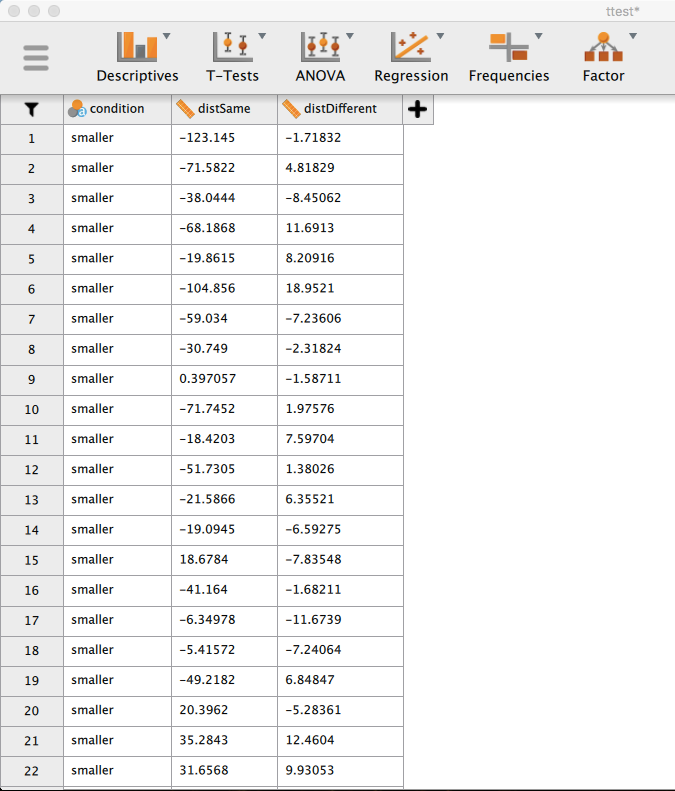
\includegraphics[width=0.65\textwidth,height=\textheight]{figures/ttestData.png}
\caption{\label{fig:ttestData}JASP screenshot showing the \texttt{ttest.csv} data set, modeled after Verguts and De Moor (2005).}
\end{figure}

Similar to Verguts and De Moor (2005), we are interested in whether the mean of the regression slopes (collapsed across participants by condition) depends on the type of decade pair being compared. As a first step, we can easily obtain some descriptive statistics. In JASP, click on the \enquote{Descriptives} in the ribbon at the top, then click \enquote{Descriptive Statistics} in the dropdown menu. This will open a dialogue box showing the list of variables available in our data set. Highlight \texttt{distSame} and \texttt{distDifferent}, then click the right-facing arrow to move these into the \enquote{Variables} box. Immediately, some descriptive statistics will appear on the right side of the screen under \enquote{Results}. To view the descriptives separately for the \enquote{Choose smaller} and \enquote{Choose larger} groups, we move the variable \texttt{condition} into the \enquote{Split} box (see Figure \ref{fig:ttestDescriptives}).

\begin{figure}
\centering
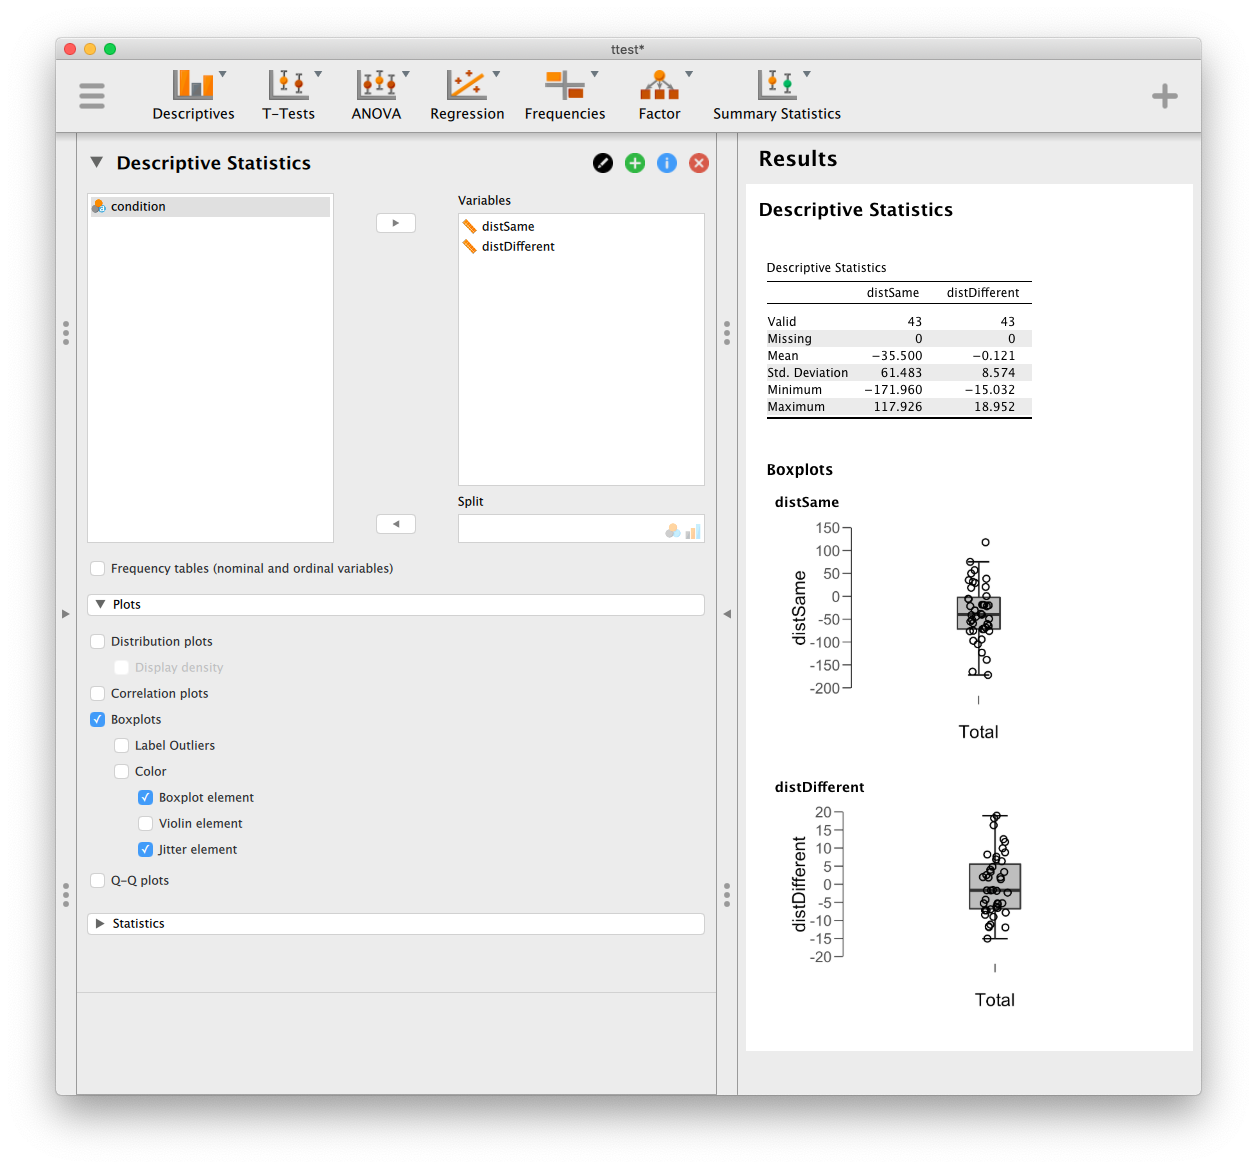
\includegraphics[width=0.9\textwidth,height=\textheight]{figures/ttestDescriptives.png}
\caption{\label{fig:ttestDescriptives}JASP screenshot showing descriptive statistics, including mean and standard deviation, for the \texttt{distSame} and \texttt{distDifferent} variables, split by \texttt{condition}.}
\end{figure}

We are now ready to perform a Bayesian analysis of the simulated Verguts and De Moor (2005) data. First, since we will separately analyze the \enquote{Choose smaller} and \enquote{Choose larger} groups, we will need to apply a \emph{filter} to the data set; specifically, we will first consider only the \enquote{Choose smaller} group. There are several ways to do this in JASP, but the easiest is the \enquote{click filter}
\footnote{For a demonstration of the different methods of filtering in JASP, see https://jasp-stats.org/2018/06/27/how-to-filter-your-data-in-jasp/.}
First, click the header of the \texttt{condition} column. To remove all of the \texttt{larger} trials from the analysis and retain only the \texttt{smaller} trials, we simply \enquote{turn off} the \texttt{larger} value by clicking on the check mark next to it. The check mark will be replaced by a cross, and you will be able to see that the \texttt{larger} trials have been greyed out. The filter dialog can be closed by clicking on the X on the right side of the dialog box. Notice that a funnel icon will appear next to the \texttt{condition} column header to indicate that a filter is currently being applied. Any filters can be removed by re-opening the filter dialog and clicking the eraser icon.

To perform a Bayesian one-sample \(t\)-test, click on the \enquote{T-Tests} button in the ribbon at the top, and select \enquote{Bayesian One Sample T-Test}. There are two \(t\)-tests that we wish to perform, but for clarity, we will start with describing one in detail. Before beginning, however, we define our two competing hypotheses explicitly. Since the numerical distance effect is expected to be negative, we define \(\mathcal{H}_{0}:\delta = 0\) and \(\mathcal{H}_{-}:\delta < 0\), where the minus in the subscript reminds us that the alternative is one-sided negative.

We will first perform a \(t\)-test for the same-decade trials. From the variable list, move \enquote{distSame} over to the \enquote{Variables} box. Since the working hypothesis states that the is negative, so we choose \enquote{\(<\) Test value} from the \enquote{Alt. Hypothesis} menu. Finally, select also \enquote{Prior and posterior} from the \enquote{Plots} menu. This setup and the resulting output appears in Figure \ref{fig:ttestBayes}. There are two components of this output that we now discuss in detail: the computed Bayes factor (top of the Results pane in Figure \ref{fig:ttestBayes}) and the plot of the prior and posterior for the effect size parameter \(\delta\) (bottom of the Results pane in Figure \ref{fig:ttestBayes}).

\begin{figure}
\centering
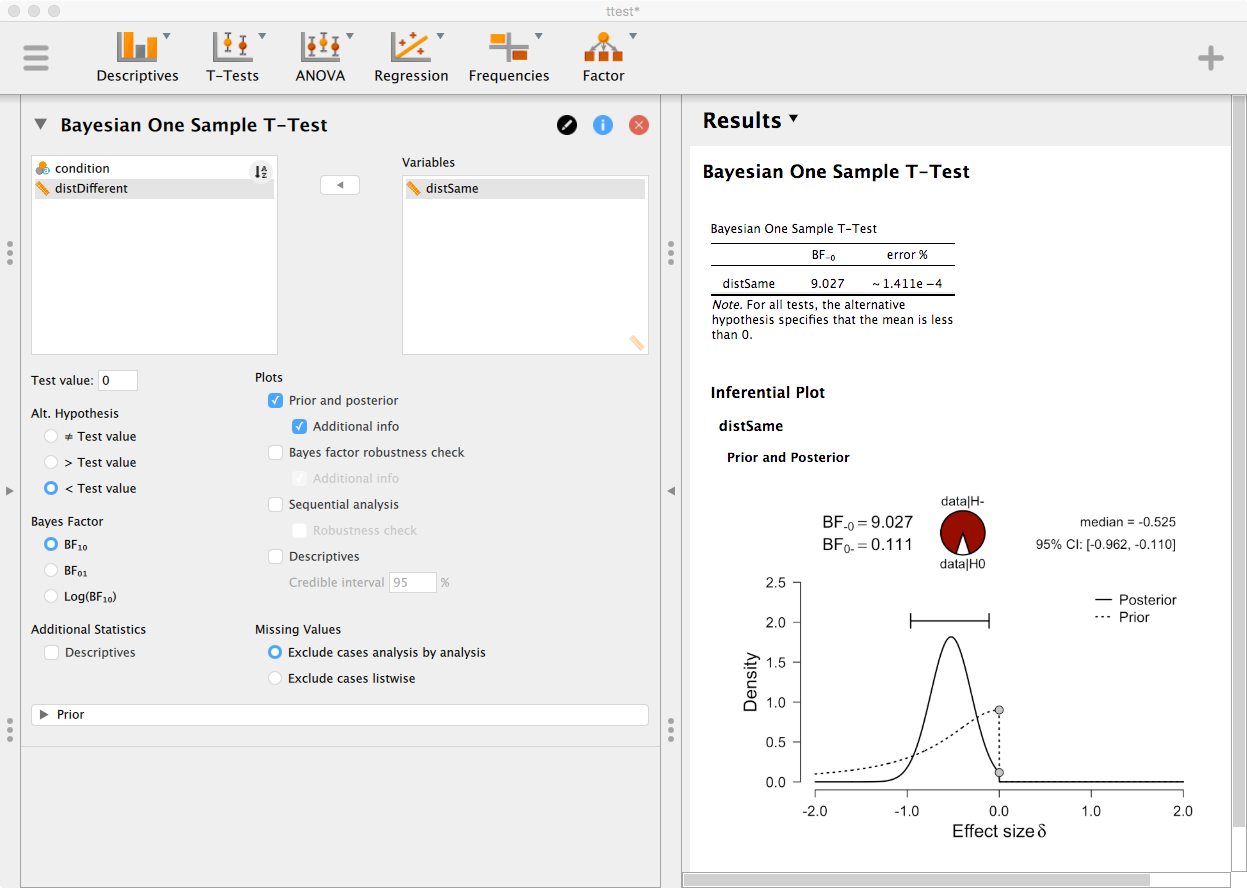
\includegraphics[width=0.9\textwidth,height=\textheight]{figures/ttestBayes.png}
\caption{\label{fig:ttestBayes}JASP screenshot showing the Bayesian one-sample \(t\)-test for \texttt{distSame}.}
\end{figure}

The Bayes factor is \(BF_{-0}=9.027\), which indicates that the observed data are approximately 9 times more likely under the alternative hypothesis \(\mathcal{H}_{1}\) than under the null hypothesis \(\mathcal{H}_{0}\). According to the convention of Jeffreys (1961), this is considered \enquote{moderate} evidence for \(\mathcal{H}_{1}\), which states that the true population effect \(\delta\) (from which our participants' regression slopes are drawn) is negative. A useful visual display of this Bayes factor is provided in the plot in the bottom of the Results pane. This probability wheel (or \enquote{pizza plot}) depicts the Bayes factor as an odds ratio of 9:027-to-1 in favor of \(\mathcal{H}_{1}\) over the null.
\footnote{To simplify matters, we identify the hypotheses to the models and use the notation \( \mathcal{H}_{k} \) interchangeably with \( \mathcal{M}_{k} \) for the \( k \)th model.}
The bottom plot shows this in more detail. The dashed line depicts the aforementioned Cauchy prior (with a default scale/prior width of \(r=1/\sqrt{2} = 0.707\)) on the population effect size \(\delta\), but restricted to negative values in accordance to the alternative \(\mathcal{H}_{-}\). The solid line depicts the posterior density for \(\delta\). Under the assumption that the effect cannot be positive, this density provides a measure of uncertainty about the size of the population effect \(\delta\) \emph{after} observing the data. We can see in Figure \ref{fig:ttestBayes} that the more probable values of \(\delta\) are now centered around \(\delta = -0.5\). For the testing problem, one specific value worth exploring is \(\delta=0\). Notice that relative to the prior, the \(y\)-coordinate at \(\delta=0\) in the posterior is smaller than the \(y\)-coordinate at \(\delta=0\). This reflects the fact that our posterior belief regarding \(\mathcal{H}_{0} : \delta = 0\) has decreased after data observation. In fact, it has decreased by a factor of approximately 9, which is the Bayes factor we obtained. This relationship is no accident; For the \(t\)-test the Bayes factor can be represented as the ratio of the prior and posterior on the population effect \(\delta\) evaluated at the null hypothesis \(\mathcal{H}_{0}: \delta = 0\). This fact is known as the Savage-Dickey density ratio (Wagenmakers, Lodewyckx, Kuriyal, \& Grasman, 2010).

In Figure \ref{fig:ttestBayes} we are also provided information about the magnitude of \(\delta\) in the form of a 95\% credible interval of {[}-0.962, -0.110{]}. This means that if the population effect is assumed to be negative --thus, under the implicit assumption that the null is false-- then with 95\% probability, the true value of the population effect \(\delta\) is between -0.962 and -0.110. Note that while it is tempting to use this estimate as a replacement for the inference that is afforded by the Bayes factor, this approach is simply not valid. The credible interval presented here is \emph{conditional on \(\mathcal{H}_{-}\)}, so it only makes sense \emph{if} \(\mathcal{H}_{-}\) is the true model. Before interpreting the credible interval, we must perform a test to index support for \(\mathcal{H}_{-}\) over \(\mathcal{H}_{0}\). So, when reporting the credible interval, we should report the Bayes factor \emph{first}, then we can report the credible interval. Do not be tempted to report the credible interval without the Bayes factor!

One last question to consider in our analysis is how sensitive the Bayes factor is to changes in the specification of the Cauchy prior on the population effect \(\delta\). Clicking the box for \enquote{Bayes factor robustness check} will help us to answer this question. Figure \ref{fig:ttestRobust} displays the result of this robustness check. As mentioned before, the default prior for \(\delta\) is a Cauchy distribution centered around \(0\) with scale (or \enquote{width}) \(r=0.707\). Figure \ref{fig:ttestRobust} depicts how the Bayes factor changes with varying values of \(r\). The plot represents the Bayes factor as a continuous function of \(r\), and the legend at the top lists the Bayes factor at four values: the value of \(r\) that produces the maximum Bayes factor, the original user-specified prior (\(r=0.707\)), a \enquote{wide} prior (\(r=1\)), and an \enquote{ultrawide} prior (\(r=\sqrt{2}=1.414\)). This plot should be interpreted holistically --across a wide range of values for the prior scale \(r\), the resulting Bayes factor ranges from 6.3 to 9, which implies that the result is quite robust.

\begin{figure}
\centering
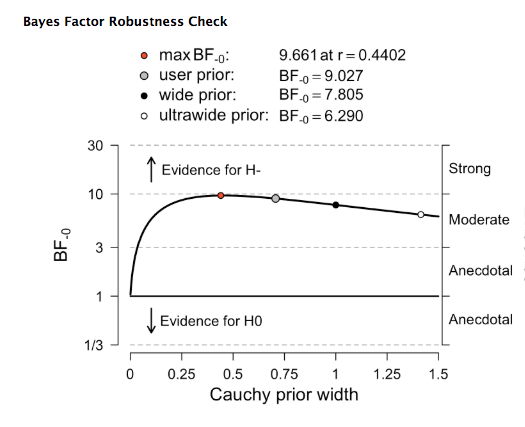
\includegraphics[width=0.6\textwidth,height=\textheight]{figures/ttestRobust.png}
\caption{\label{fig:ttestRobust}JASP screenshot showing a Bayes factor robustness check for the one-sample \(t\)-test on \texttt{distSame}.}
\end{figure}

Now we are ready to perform a Bayesian \(t\)-test for the different-decade trials. Recall that these were the critical trials for Verguts and De Moor (2005), as a null numerical distance effect would lend support for a strictly decomposed model of two-digit number processing. We perform this test in an identical manner to the previous test, with one exception. After moving the variable \texttt{distDifferent} to the \enquote{Variables} list, we select \(\textnormal{BF}_{01}\) from the \enquote{Bayes Factor} menu. Note that this is not strictly necessary to perform the analysis, but doing so will cast our Bayes factor in terms of support for our working hypothesis \(\mathcal{H}_{0}\) over \(\mathcal{H}_{-}\). The result is shown in Figure \ref{fig:ttestBayes2}. We obtain \(\textnormal{BF}_{0-}=7.595\), indicating that our data are approximately 7.5 times more likely under \(\mathcal{H}_{0}\) than \(\mathcal{H}_{-}\). This shows some evidence that the true population effect \(\delta\), from which our synthethic data were generated, is equal to 0. As we can see in Figure \ref{fig:ttestBayes2}, our posterior belief that \(\delta=0\) has \emph{increased} relative to our prior belief that \(\delta=0\), specifically by a factor of 7.595.

\begin{figure}
\centering
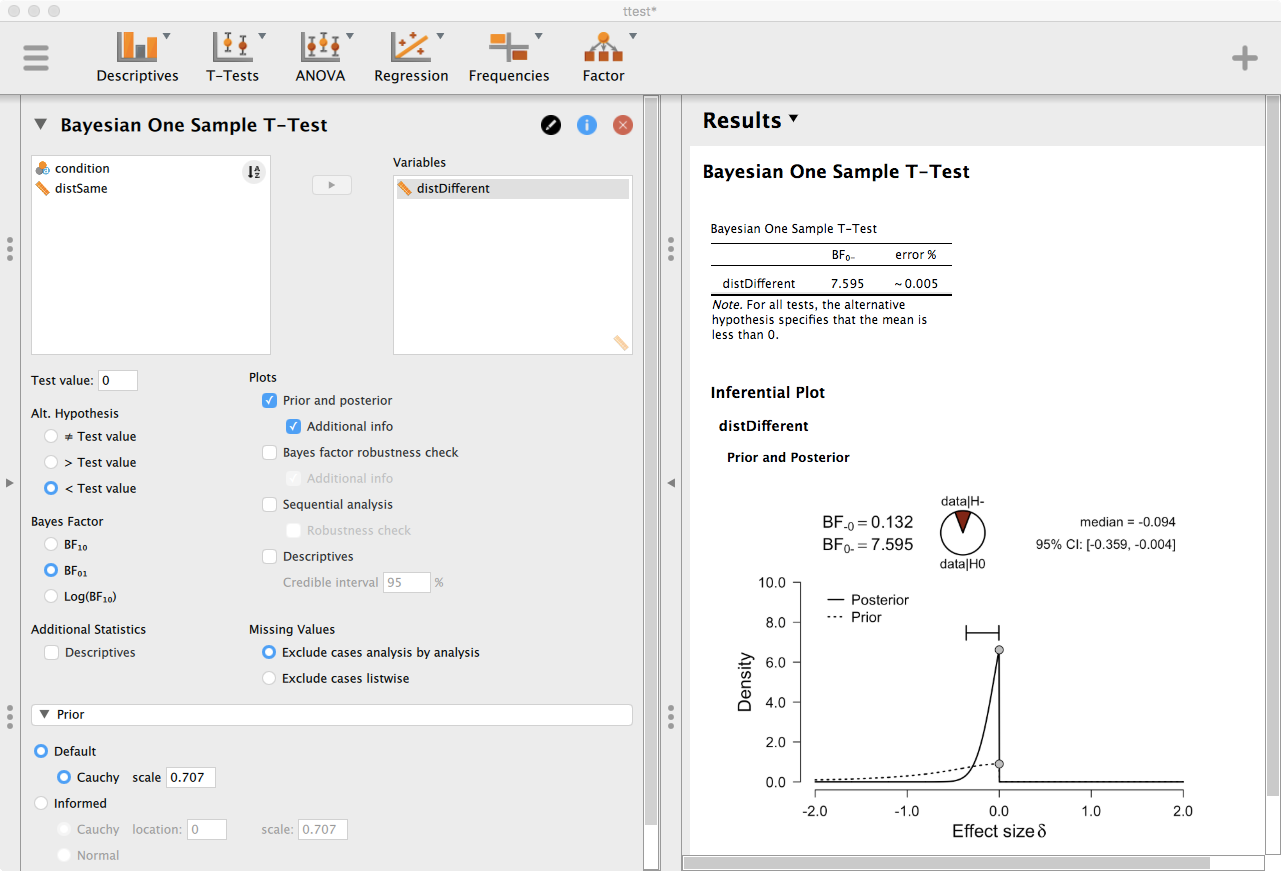
\includegraphics[width=0.9\textwidth,height=\textheight]{figures/ttestBayes2.png}
\caption{\label{fig:ttestBayes2}JASP screenshot showing a Bayesian one-sample \(t\)-test for the \texttt{distDifferent} variable.}
\end{figure}

It is again important to note that the 95\% credible interval that is displayed in the figure is conditional on \(\mathcal{H}_{-}\). In other words, it only makes sense if \(\mathcal{H}_{-}\) is the true model. However, in this case, we have moderate evidence that \(\mathcal{H}_{0}\) is the true model, so we can ignore this credible interval. Conditioned on the null \(\mathcal{H}_{0}\) our best guess for size of the effect would simply be \(\delta = 0\). It is also worth mentioning that there might be some confusion present when to take this credible interval at face value. Some might argue that since the credible interval does not contain 0 (its right endpoint is -0.004), this is actually evidence for \(\mathcal{H}_{-}\). However, this is simply not true. The apparent paradox lies in how the credible interval is computed; in JASP the 95\% credible interval is computed as the \emph{central} 95\% of the mass of the posterior for \(\delta\). Since there is no posterior mass to the right of \(\delta=0\), this central portion of the posterior must necessarily be contained strictly to the left of \(\delta=0\), thus producing the right end point that is slightly less than \(\delta=0\). However, if we were to instead specify the credible interval as 95\% of the posterior distribution with \emph{highest density}, the resulting credible interval would contain \(\delta=0\). Currently, this functionality is not available in JASP, so great care must be taken in interpreting the credible interval for \(\delta\) based on restricted priors.

What is important to realize is that a test addresses a different question than an estimation. The Bayes factor focuses on the question \enquote{Does the effect exist?}, whereas the posterior focuses on the question \enquote{If it exists, then how large is it?}. This is why the (Bayesian) testing problem compares the model where the population effect is fixed at zero against one where it is free to vary. Once the data have convinced us that the population effect \(\delta\) varies freely, only then would we be interested in the magnitude of the effect.

We can follow the same steps described above on the participants who were assigned to the \enquote{choose larger} condition. The inference is largely the same. For same decade trials, we obtain \(\textnormal{BF}_{-0}=7.543\), indicating that the data are approximately 7.5 times more likely under \(\mathcal{H}_{-}\) than under \(\mathcal{H}_{0}\). This provides some evidence that the true population effect \(\delta\) is negative, which is indicative of a negative numerical distance effect. For different decade trials, the inference is less clear; we obtain \(\textnormal{BF}_{0-}=1.893\), indicating that the observed data are approximately 2 times more likely under \(\mathcal{H}_{0}\) than under \(\mathcal{H}_{-}\). The progression of the Bayes factor is visualized in Figure \ref{fig:ttestSequential}, which was obtained by selecting the \enquote{Sequential analysis} option. This plot shows how the Bayes factor changes sequentially as each data point is added, starting from \(\textnormal{BF}_{0-}=1\) (no preference for either model) at \(n=1\) to the obtained Bayes factor of \(\textnormal{BF}_{01}=1.893\) at \(n=20\). As can be seen in Figure \ref{fig:ttestSequential}, the incoming data were first better predicted by \(\mathcal{H}_{-}\) than by \(\mathcal{H}_{0}\), with the Bayes factor \enquote{crossing over} to support for \(\mathcal{H}_{0}\) at the 20th participant. Certainly, this shows that we should be quite reserved about our conclusions at this point. In fact, if these were real data, we might prefer to continue sampling additional participants until the Bayes factor stabilizes. In general, when the population effect is truly non-zero the Bayes factor in favor of the alternative grows fast (i.e., exponentially in \(n\)). On the other if the population effect is actually zero, then the evidence for the null grows slowly (i.e., as a square root in \(n\)); see for instance Bahadur and Bickel (2009) and Johnson and Rossell (2010).

\begin{figure}
\centering
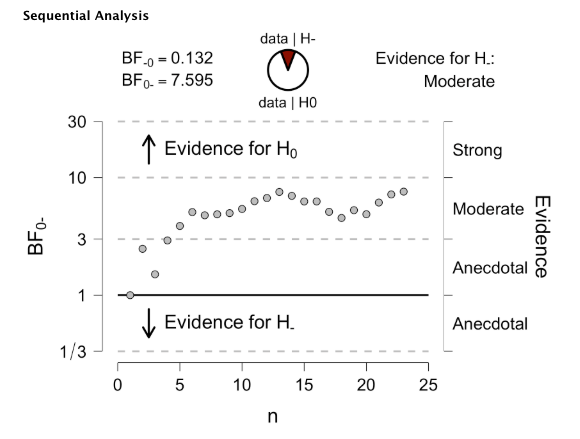
\includegraphics[width=0.6\textwidth,height=\textheight]{figures/ttestSequential.png}
\caption{\label{fig:ttestSequential}JASP screenshot showing a sequential analysis.}
\end{figure}

\hypertarget{example-2-a-bayesian-linear-regression}{%
\section{Example 2: a Bayesian linear regression}\label{example-2-a-bayesian-linear-regression}}

We use an example inspired by Holloway and Ansari (2009), who examined the relationship between basic numerical processing and higher mathematical skills in children. Specifically, they examined whether childrens' mathematical achievement scores were related to their ability to compare symbolic and nonsymbolic number magnitudes. In this example, we will recreate one specific component of their analysis; namely, we will use Bayesian linear regression to examine the extent to which mathematical fluency scores are predicted by childrens' standardized symbolic and nonsymbolic distance effects. To operationalize these effects, Holloway and Ansari (2009) subtracted the mean RT for large numerical distances from the mean RT for small numerical distances, and then standardized across individuals by dividing the resulting RT difference by the mean RT for large distances.
In their original paper, Holloway and Ansari (2009) found that the childrens' symbolic distance effect was a significant predictor of fluency, \(\beta = -0.236\), \(p<0.05\), whereas the nonsymbolic distance effect did not predict fluency, \(\beta=0.063\), \(p > 0.05\).

The questions we would like to address here are (1) \enquote{Which out of these two covariates (\(x_{1}=\text{ symbolic distance effect}\) and \(x_{2}=\text{ nonsymbolic distance effect}\)) predict fluency score?}, and (2) \enquote{How large is the effect \(\beta_{i}\) of each covariate \(x_{i}\)?}. Note that the first question can be answered by: (a) neither symbolic nor nonsymbolic, (b) only symbolic, (c) only nonsymbolic, and (d) both symbolic and nonsymbolic distance effects predict fluency score. Equivalently, these answers correspond to specific hypotheses about the regression coefficients \(\beta_{i}\), namely: (a') the coefficients for both symbolic and nonsymbolic are equal to 0; (b') only the coefficient for nonsymbolic is equal to zero; (c') only the coefficient for symbolic is equal to zero; and (d') neither coefficient is equal to zero. Cast in this manner, the first question is the testing problem, whereas the second question deals with the estimation problem.

\hypertarget{theory-of-bayesian-linear-regression}{%
\subsection{Theory of Bayesian linear regression}\label{theory-of-bayesian-linear-regression}}

\hypertarget{linear-regression-models}{%
\subsubsection{Linear regression models}\label{linear-regression-models}}

As with the \(t\)-test, the technical details described here are included for completeness, but are not strictly necessary for the remainder of this section. We first elaborate on linear regression models, before we discuss the Bayesian implementation.

We write \(Y_{i}\) for the continous outcome variable of the \(i\)th participant, and \(x_{i1}, x_{i2}, \ldots, x_{ip}\) for the \(i\)th participant's covariates. For the example at hand, \(Y_{i}\) represents a participant's mathematical fluency score, and we have \(p=2\) covariates consisting of the \(i\)th participant's measurements \(x_{i1}=\text{ symbolicDE}_{i}\), and \(x_{i2}=\text{ nonsymbolicDE}_{i}\).

The difficulty here is that with \(p\) covariates there are \(2^{p}\) models. For instance with \(p=2\), we have \(2^{p} = 4\) models, which are given by
\begin{align*}
\mathcal{M}_{0} & : Y_{i} =\beta_{0} + \varepsilon_{i}, \\
\mathcal{M}_{1} & : Y_{i} =\beta_{0} + \beta_{1} x_{i1} + \varepsilon_{i}, \\
\mathcal{M}_{2} & : Y_{i} =\beta_{0} + \beta_{2} x_{i2} + \varepsilon_{i}, \\
\mathcal{M}_{3} & : Y_{i} =\beta_{0} + \beta_{1} x_{i1} + \beta_{2} x_{i2} + \varepsilon_{i},
\end{align*}
where \(\beta_{0}\) represents the intercept, \(\beta_{1}\) the effect of symbolicDE on \(Y_{i}\), \(\beta_{2}\) the effect of nonsymbolicDE on \(Y_{i}\), and \(\varepsilon_{i} \sim \mathcal{N}(0, \sigma^{2})\) is a normally distributed error. Each model can be thought of as an operationalisation of a hypothesis. Note that all models include the intercept and error variance \(\sigma^{2}\) parameters, which are related to the outcome variable \(Y_{i}\). The models \(\mathcal{M}_{0},\mathcal{M}_{1},\mathcal{M}_{2}, \mathcal{M}_{3}\) have 2, 3, 3 and 4 parameters, respectively. In general, the largest model will have \(p + 2\) parameters.

All models decompose \(Y_{i}\) into two parts: a part that is structural, and a part that is simply noise. For the null model, all the structure is given by the intercept \(\beta_{0}\), whereas in \(\mathcal{M}_{1}, \mathcal{M}_{2}\) and \(\mathcal{M}_{3}\) the intercept \(\beta_{0}\) competes with the covariates to predict \(Y_{i}\). Hence, despite terms being denoted with the same symbol, such as the intercepts \(\beta_{0}\), they have a different impact on \(Y_{i}\) depending on the context given by the model. As such, the question whether symbolicDE has an effect on fluency depends on the particular model that is being compared.

\hypertarget{bayesian-linear-regression}{%
\subsubsection{Bayesian linear regression}\label{bayesian-linear-regression}}

To avoid this problem, we exploit the flexibility of Bayesian methods, and address questions such as whether symbolicDE has an effect on fluency by averaging across all models considered. To model average we require weights, and for simplicity we assume that all models are equally probable a priori. In other words, we put a uniform prior on the models, and because we have four models each model gets a prior model probability of \(1/4=0.25\). Table \ref{tabLinreg} provides a summary of this information.

\begin{table}
\label{tabLinreg}
\caption{List of all models with the two potential predictors and the prior model probability of each model. A "1" indicates that the predictor is active in model, whereas a "0" implies that the predictor is inactive.}
\begin{center}
\begin{tabular}{rllll}
\hline
Model & symbolicDE & nonsymbolicDE & \( P(\mathcal{M}) \) \\
\hline
\( \mathcal{M}_{0} \) & 0 & 0 & 0.25 \\
\( \mathcal{M}_{1} \) & 1 & 0 & 0.25 \\
\( \mathcal{M}_{2} \) & 0 & 1 & 0.25 \\
\( \mathcal{M}_{3} \) & 1 & 1 & 0.25 \\
\hline
\end{tabular}
\end{center}
\end{table}

The a priori probability of the relevance of the covariate symbolicDE on \(Y_{i}\) is given by aggregating the probabilities of the models \(\mathcal{M}_{1}\) and \(\mathcal{M}_{3}\), thus, 50\%. Similarly, the a priori relevance of the covariate nonsymbolicDE is also 50\%, whereas the a priori probability of both symbolicDE and nonsymbolicDE having an impact on \(Y_{i}\) is only given by \(P(\mathcal{M}_{3}) = 0.25\).

To compute the relevance of each covariate \textbf{after} data observation, we simply replace the prior model probabilities in the table by the posterior model probabilities. These are calculated using a generalisation of Equation \eqref{eqPriorToPosterior} which specifies that the posterior model probability for model \(k=0, 1, \ldots p-1 = 3\) is given by
\begin{equation}
\label{eqPriorToPosteriorGeneral}
P(\mathcal{M}_{k} \mid d) = \frac{ \textnormal{BF}_{k0}(d) P(\mathcal{M}_{k})}{ \sum_{k=0}^{p-1} \textnormal{BF}_{k0}(d) P(\mathcal{M}_{k})},
\end{equation}
where the comparison between the null model and itself is defined as \(\textnormal{BF}_{00}(d) = 1\) regardless of the data. Now, suppose that the model \(\mathcal{M}_{k}\) has \(l \leq p\) active covariates. Then for the Bayes factor \(\textnormal{BF}_{k0}\), we need to choose a prior on \(l + 2\) parameters for \(\mathcal{M}_{k}\) and a prior on \(2\) parameters for \(\mathcal{M}_{0}\). Zellner and Siow (1980) proposed to use essentially the same priors Jeffreys used for his Bayesian \(t\)-test. This connection is made explicit by exploiting the assumption of normally distributed errors to rewrite the linear regression models as the following normal means models:
\begin{align}
\label{eqLinRegAsNormal0}
\mathcal{M}_{0} & : Y_{i} \, | \, x_{i} \sim \mathcal{N}(\beta_{0}, \sigma^{2}), \\
\mathcal{M}_{1} & : Y_{i} \, | \, x_{i} \sim \mathcal{N}(\beta_{0} + \beta_{1} x_{i1}, \sigma^{2}), \\
\mathcal{M}_{2} & : Y_{i} \, | \, x_{i} \sim \mathcal{N}(\beta_{0} + \beta_{2} x_{i2}, \sigma^{2}), \\
\label{eqLinRegAsNormal3}
\mathcal{M}_{3} & : Y_{i} \, | \, x_{i} \sim \mathcal{N}(\beta_{0} + \beta_{1} x_{i1} + \beta_{2} x_{i2} , \sigma^{2}),
\end{align}
where \(Y_{i} \, | \, x_{i}\) refers to the outcome variable given the covariates \(x_{i}\).

More explicitly, the Bayes factor \(\textnormal{BF}_{k0}\), where \(\mathcal{M}_{k}\) has \(l\) active covariates, uses an \enquote{uninformative} prior on the nuisance parameter \(\beta_{0}\) and \(\sigma\) in both models, and for the \(\mathcal{M}_{k}\) an additional \(l\)-dimensional multivariate Cauchy prior on the vector of population effect sizes \(\delta\). The vector of effect sizes is defined by rescaling the vector of active \(\beta\) coefficients with respect to \(\sigma\), but also with respect to the covariates. More explicitly, when \(l=1\), say, only \(\beta_{2}\) is active then the effect size parameter is given by \(\delta = \beta_{2} s_{x_{2}}/\sigma\), where \(s_{x_{2}}\) is observed standard error of the second covariate. If the second covariate is standardised, then \(s_{x_{2}} = 1\), and we get the same definition of effect size as in the \(t\)-test, but with \(\mu\) replaced by \(\beta_{2}\). Furthermore, with \(l = 1\), the prior on \(\delta\) is than a \(1\)-dimensional Cauchy distribution, indeed, the same one we would use in the \(t\)-test.

The rescaling with respect to the covariates is necessary to make the Bayes factor independent of the unit of measurements of the covariates. Similarly, the uninformative priors on \(\beta_{0}\) and \(\sigma\) are needed to make the Bayes factor independent of the unit of measurement of \(Y_{i}\). The Bayes factors for linear regression also retains other desirable properties of the Bayesian \(t\)-test; see Rouder and Morey (2012), Liang et al. (2008) and Bayarri et al. (2012) for more details, and Li and Clyde (2018) for further extensions.

With both the prior model probabilities and the Bayes factor at hand \eqref{eqPriorToPosteriorGeneral} now provides the posterior model probabilities. Once the latter are computed, the posterior relevance of each covariate can be assessed as we have done in Table \ref{tabLinreg}. We elaborate on this procedure with the example.

\hypertarget{implementation-in-jasp-1}{%
\subsection{Implementation in JASP}\label{implementation-in-jasp-1}}

After downloading the file \texttt{regression.csv} from the Github repository (\url{https://git.io/JeXui}), open the file in JASP. This will reveal a data set with three variables: \texttt{symbolicDE}, representing the standardized distance effect measure for the symbolic number comparison task; \texttt{nonsymbolicDE}, representing the standardized distance effect measure for the nonsymbolic comparison task; and \texttt{fluency}, representing the mathematics fluency score.

To perform the Bayesian linear regression, we click the \enquote{Regression} button and select \enquote{Bayesian Linear Regression}. We then move the \texttt{fluency} variable to the \enquote{Dependent Variable} box and we move both the \texttt{symbolicDE} and \texttt{nonsymbolicDE} variables to the \enquote{Covariates} box. We will leave the basic defaults in place except for two. First, select \enquote{Posterior summary} under \enquote{Output}. Also, we will select one more option that is found in the \enquote{Advanced Options}, but will actually simplify our discussion for this tutorial. Under \enquote{Model Prior}, select \enquote{Uniform}. The output can be seen in Figure \ref{fig:regression1}.

\begin{figure}
\centering
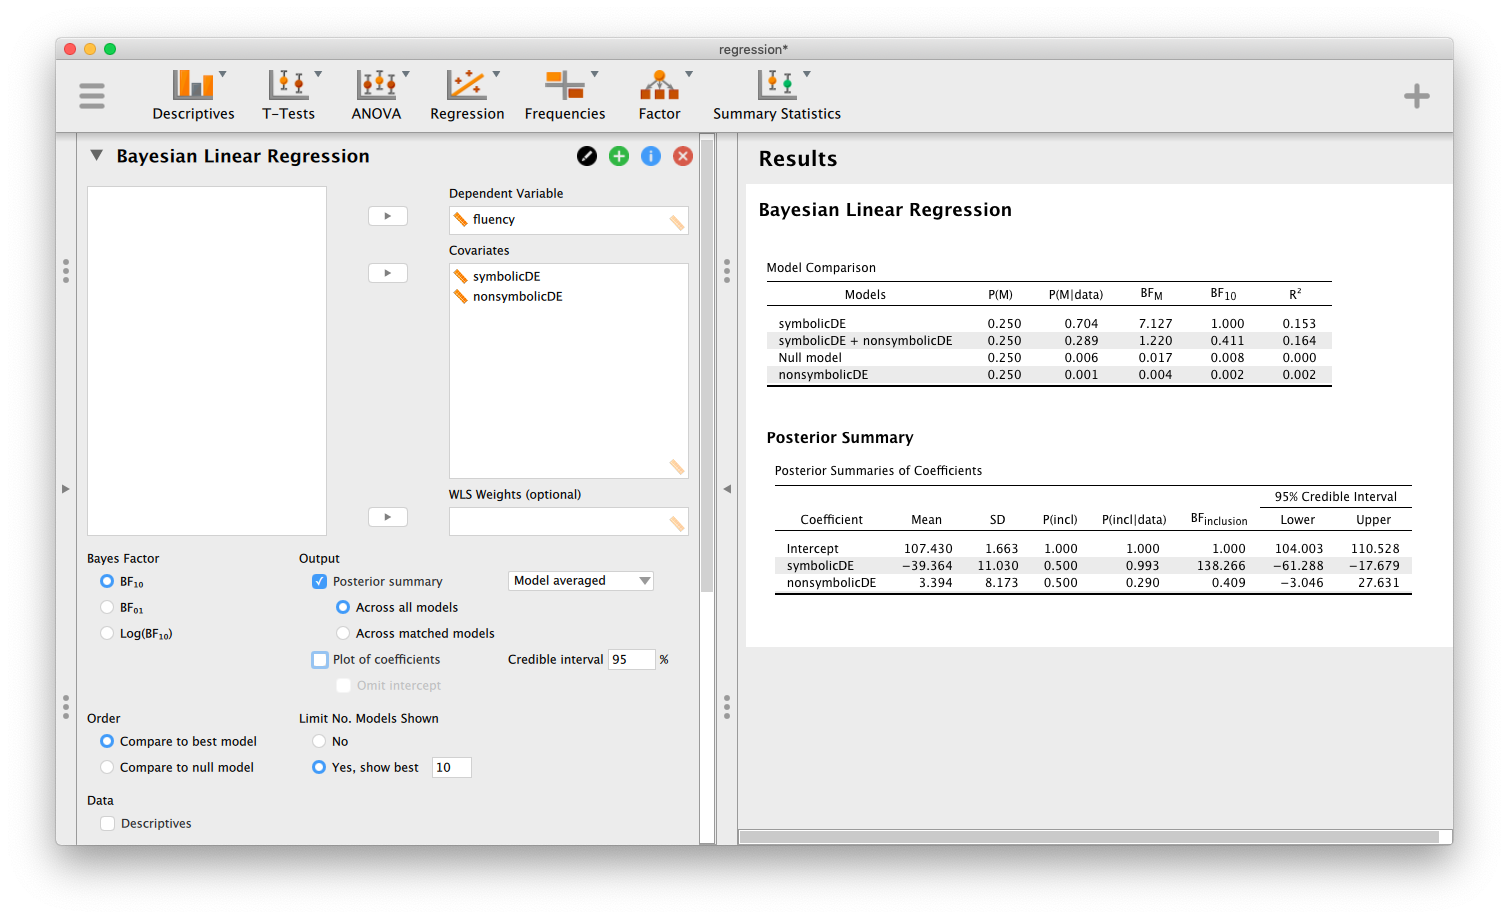
\includegraphics[width=0.9\textwidth,height=\textheight]{figures/regression1.png}
\caption{\label{fig:regression1}JASP screenshot showing a Bayesian linear regression.}
\end{figure}

First, we will walk through the basic output given by JASP. As can be seen in the output table in Figure \ref{fig:regression1}, JASP constructs four models with the two possible predictor variables:
\begin{align*}
\mathcal{M}_{0}: & \text{ fluency} = \text{Null model} \\
\mathcal{M}_{1}: & \text{ fluency} = \text{symbolicDE} \\
\mathcal{M}_{2}: & \text{ fluency} = \text{nonsymbolicDE} \\
\mathcal{M}_{3}: & \text{ fluency} = \text{symbolicDE}+\text{nonsymbolicDE}
\end{align*}
These models are each displayed in the rows of the output in Figure \ref{fig:regression1} in decreasing order of posterior model probability (i.e., the model with the highest posterior model probability is listed at the top). We can see immediately that the best model is \(\mathcal{M}_{1}\), which posits that fluency is predicted only by the symbolic distance effect. But, to understand why it is the best model and how it compares to the other 3 models, we need to discuss what each of the columns in the output table represent.

The first column, \(P(M)\), lists the prior probabilities of the 4 models. Above, we specified that the prior model probabilities should be uniform. Under this option, JASP gives the models equal prior model probability. Since there are 4 models, the prior probability of each model is \(1/4 = 0.25\). The second column, \(P(M \mid \text{data})\), gives the posterior model probabilities. Like the prior model probabilities, these must add to 1, but now there has been some shift from prior model probability to posterior model probability. Here, after observing data, we can see that \(\mathcal{M}_{1}\) and \(\mathcal{M}_{3}\) account for most of our posterior belief, with posterior probabilities 0.704 and 0.289, respectively. The remaining two models have very low posterior probability totalling 0.007.

Various Bayes factors are contained in the third and fourth columns. Each column gives a slightly different type of Bayes factor, however, and must be interpreted appropriately. The third column, \(\textnormal{BF}_{M}\), gives the factor by which the prior odds for a given model have been updated to produce the posterior odds for that model. For example, consider \(\mathcal{M}_{1}\), the model where fluency is predicted only by the symbolic distance effect. The prior odds for \(\mathcal{M}_{1}\), which is defined as the probability that \(\mathcal{M}_{1}\) is the true model divided by the probability that \(\mathcal{M}_{1}\) is \emph{not} the true model, can be computed as \(0.25/(1-0.25) = 0.25/0.75 = 0.333\). By similar calculation, the posterior odds are equal to \(0.704/(1-0.704) = 0.704/0.296 = 2.378\). Thus, the updating factor from prior odds to posterior odds is calculated as \(2.378/0.333 = 7.127\). One of the useful properties of this column is that it tells the user quickly whether the odds for a particular model has \emph{increased} or \emph{decreased}. As we can see in Figure \ref{fig:regression1}, the data has increased model odds for both \(\mathcal{M}_{1}\) and \(\mathcal{M}_{3}\), but only just slightly for \(\mathcal{M}_{3}\).

Finally, the fourth column, \(\textnormal{BF}_{10}\), lists the Bayes factor for a given model compared to the most probable model (note that this is the default setting in JASP, but if desired, it can be changed by the user to instead display the Bayes factor compared to the null model).
\footnote{It is easy to compute the Bayes factor with respect to the most probable model, once we have the Bayes factor with respect to the null model. Let \( \textnormal{BF}_{10}, \textnormal{BF}_{20}, \textnormal{BF}_{30} \) be the Bayes factors with respect to the null model. Recall that in our case model \( \mathcal{M}_{1} \) is the best model. The Bayes factor \( \textnormal{BF}_{31} =\textnormal{BF}_{30} \textnormal{BF}_{01} \), where \( \textnormal{BF}_{01}= 1/\textnormal{BF}_{10} \).}
This is a very useful column for doing specific model comparisons. For example, we can use this column to directly compare the two most probable models, \(\mathcal{M}_{1}\) and \(\mathcal{M}_{3}\). In the results table, we see that the Bayes factor for the \(\mathcal{M}_{3}\) compared to the best fitting model \(\mathcal{M}_{1}\) is 0.411. Taking reciprocals, this tells us that the Bayes factor for \(\mathcal{M}_{1}\) over \(\mathcal{M}_{3}\) is \(1/0.411 = 2.43\). In other words, the observed data are approximately 2.5 times more likely under the model where fluency is predicted only by the symbolic distance effect compared to the model where fluency is predicted by both symbolic and nonsymbolic distance effects. Another way of saying this is that we have positive evidence for excluding nonsymbolic distance effect as a predictor of mathematical fluency once we already accepted symbolic distance effect as a predictor.

Once we have positive evidence for \(\mathcal{M}_{1}\), which posits only symbolicDE as a predictor of fluency, we can move to the problem of estimation. To this end, we focus on two outputs: (1) the \enquote{Posterior Summary} output of Figure \ref{fig:regression1}; and (2) the \enquote{Marginal posterior distributions} plot (see Figure \ref{fig:marginalPosterior}), which can be displayed by clicking on the \enquote{Plots} menu in JASP. Both outputs provide model averaged posterior summaries of the regression coefficients \(\beta_{0}\) (the intercept), \(\beta_{1}\) (the coefficient of symbolicDE), and \(\beta_{2}\) (the coefficient of nonsymbolicDE). Before interpreting these outputs, however, there are some subtle details that we should discuss. As mentioned earlier in the \(t\)-test example, any estimation that we present is conditional on \emph{some} model. However, in this example, we have four models to consider. So, how to proceed? One approach is to employ Bayesian model averaging, which JASP performs by default. Basically, it works as follows. Rather than estimating a parameters conditioned on one specific model, JASP calculates an \emph{average} posterior distribution for the parameter. That is, we factor in both the uncertainty about the parameter within any one particular model \emph{and} the uncertainty about the models themselves. We think this is a good approach to estimation, as it alleviates the need for the researcher to pick one model as \enquote{the winner}, and instead, provides estimates that incorporate both levels of uncertainty (within models and across models).

\begin{figure}
\centering
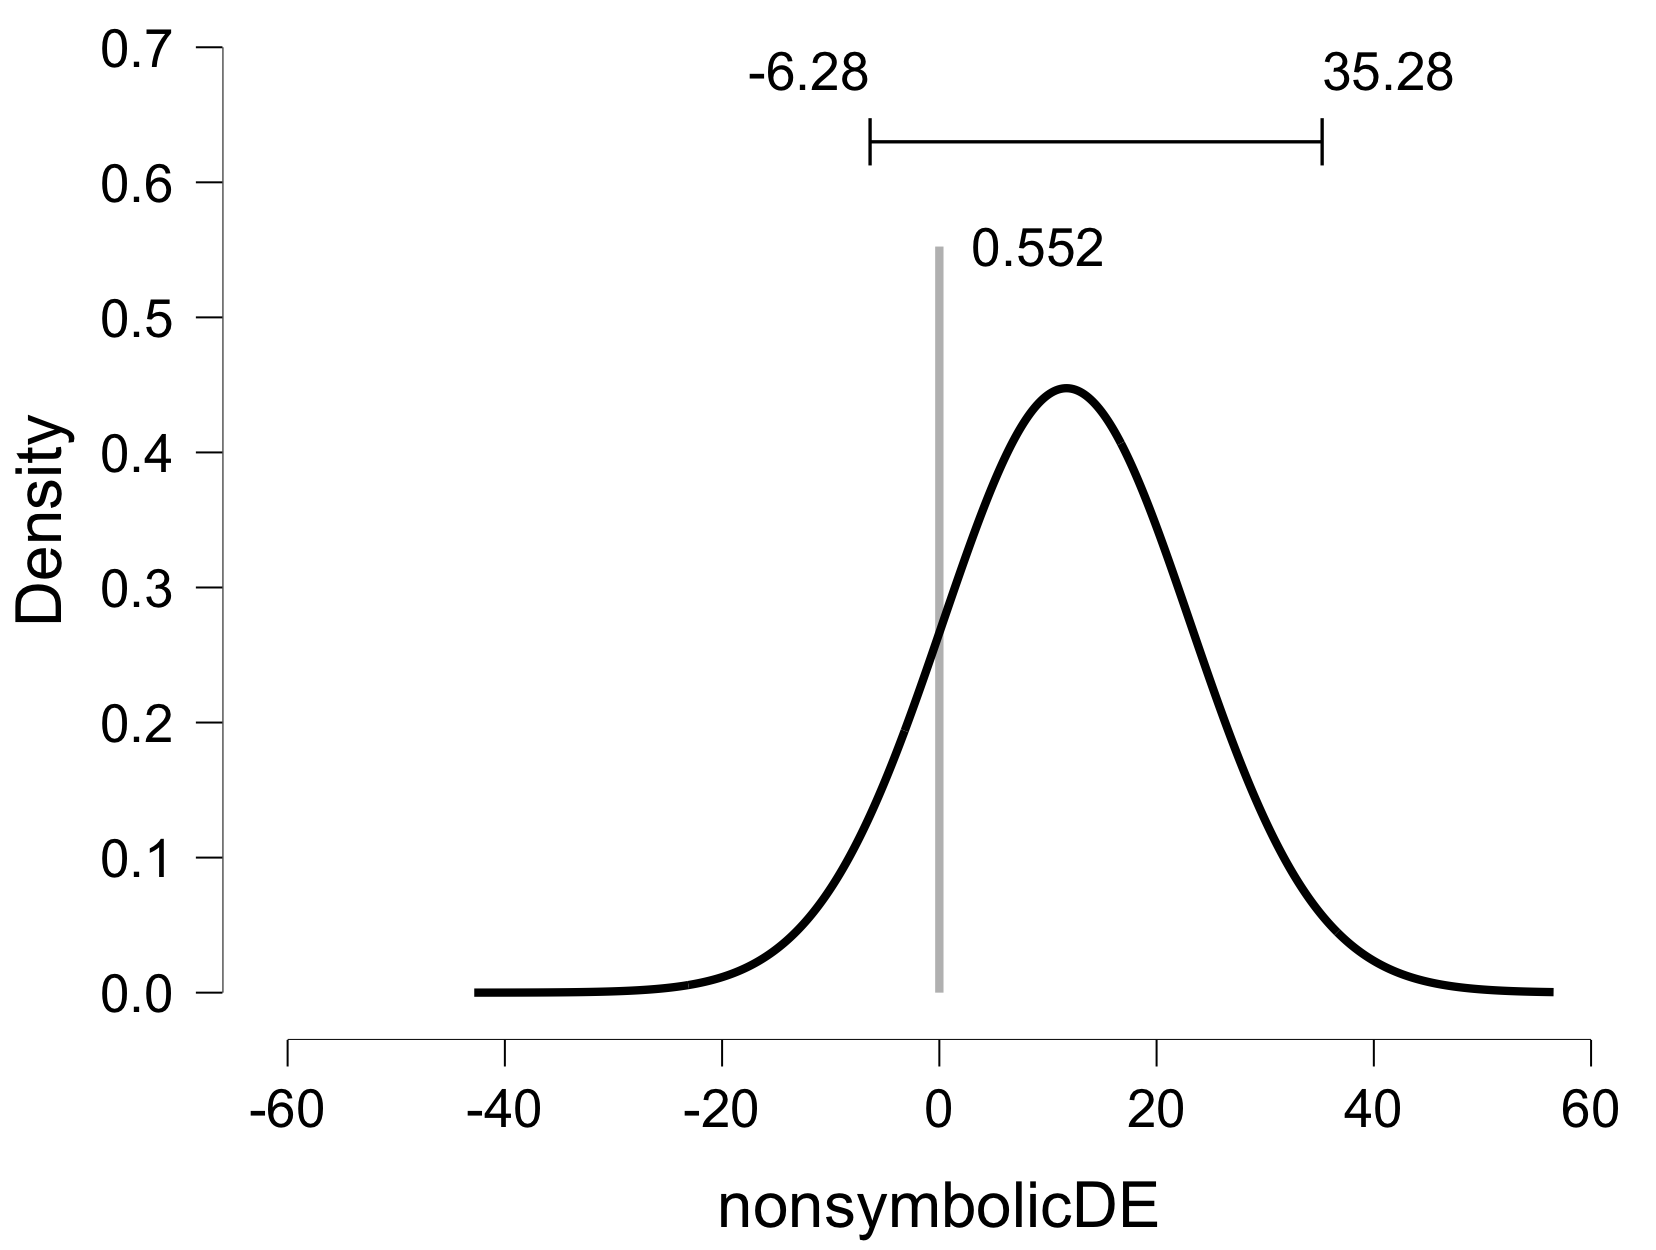
\includegraphics[width=0.6\textwidth,height=\textheight]{figures/marginalPosterior.png}
\caption{\label{fig:marginalPosterior}JASP screenshot showing the marginal posterior distribution for the nonsymbolicDE predictor in our linear regression example. The \enquote{spike} at zero with 0.552 represents the posterior model probability that the coefficient is zero.}
\end{figure}

Given this background, let us first interpret the Posterior Summary table in Table \ref{fig:regression1}. First, the table provides estimates of mean and standard deviation for the three coefficients, as well as 95\% credible intervals. Moreover, the table provides \enquote{inclusion probabilities}, which provide prior and posterior probabilties of including each covariate as a predictor of the linear model. We can take a look at these in more detail. First, let us focus on \(P(\text{incl})\), the prior inclusion probability for each covariate. These are based on the prior model probabilities that we chose in Table \ref{tabLinreg}. Since the intercept \(\beta_{0}\) was included in each of the 4 models, and each model \(\mathcal{M}_{k}\) had prior probability 0.25, the prior probability of including the intercept \(\beta_{0}\) is equal to \(4(0.25) = 1\). On the other hand, only two of the models (\(\mathcal{M}_{1}\) and \(\mathcal{M}_{3}\)) included the covariate symbolicDE. Since each of these models had prior probability 0.25, the prior probability of including the predictor symbolicDE is equal to \(2(0.25) = 0.5\). A similar argument shows the same prior probability for the covariate nonsymbolicDE.

After observing data, we can calculate the posterior inclusion probabilities \(P(\text{incl}\mid \text{data})\). This can be done easily by considering the posterior probability of each model in the \enquote{Model Comparison} table of Figure \ref{fig:regression1}. The intercept is in each of the models, so summing the posterior probabilities for all four models produces \(P(\text{incl}\mid \text{data}) = 1\). For symbolicDE, we sum the posterior probabilities for \(\mathcal{M}_{1}\) and \(\mathcal{M}_{3}\), which gives \(P(\text{incl}\mid \text{data}) = 0.704 + 0.289 = 0.993\). Finally, for nonsymbolicDE, we sum the posterior probabilities for \(\mathcal{M}_{2}\) and \(\mathcal{M}_{3}\), giving \(P(\text{incl}\mid \text{data}) = 0.289 + 0.001 = 0.290\).

Using these posterior inclusion probabilities, we can calculate an \enquote{inclusion Bayes factor}, which is defined as the factor by which the prior odds for including a specific predictor are increased after observing data. For example, the prior odds for including symbolicDE is equal to 0.5/(1-0.5) = 1, and the posterior odds is equal to 0.993/(1-0.993) = 138.27. Thus, the odds have increased by a factor of 138.27/1 = 138.27. Similarly, the prior odds for including nonsymbolicDE as a predictor is equal to 1, whereas the posterior odds is equal to 0.290/(1-.290) = 0.409. We can interpret this Bayes factor less than one via the reciprocal by reporting that the odds of including have \emph{decreased} after observing data by a factor of 1/0.409 = 2.45.

Finally, let us consider the marginal posterior distribution displayed in Figure @ref\{fig:marginalPosterior\}. For simplicity of discussion, we only display the marginal posterior for the nonsymbolicDE covariate, though JASP provides a plot for each covariate being considered. The figure shows exactly what is meant by model averaging; from the discussion above, we know there is uncertainty about whether to include nonsymbolicDE as a predictor in the overall model. This uncertainty can be quantified as the posterior inclusion probability, which from the posterior summary table we know to be \(P(\text{incl}\mid \text{data}) = 0.448\). Thus, it easily follows that the posterior probability of \emph{excluding} nonsymbolicDE as a predictor is \(1-0.448 = 0.552\); this probability is displayed in Figure \ref{fig:marginalPosterior} as a \enquote{spike} at 0. This spike together with with the posteriors of each model result in an unconditional 95\% credible interval, which states that the coefficient for nonsymbolicDE ranges from -6.28 to 35.28.

\hypertarget{example-3-a-factorial-analysis-of-variance}{%
\section{Example 3: A factorial analysis of variance}\label{example-3-a-factorial-analysis-of-variance}}

In our final example, we demonstrate a Bayesian factorial analysis of variance. To do this, we use a data set based on Campbell and Fugelsang (2001), who investigated the effects of problem size and numerical surface form on response times in an addition verification task. Not only did they find the usual effects of problem size (small problems are solved faster than large problems) and problem format (digit problems are solved faster than word problems), but they also observed an interaction between size and format; specifically, the problem size effect was larger for problems in word format than for problems in digit format. This interaction was interpreted as support for an \emph{interaction} model of mental arithmetic, where factors that influence encoding processes (e.g., surface format) also directly influence calculation processes.

\hypertarget{theory-of-bayesian-analysis-of-variance}{%
\subsection{Theory of Bayesian analysis of variance}\label{theory-of-bayesian-analysis-of-variance}}

The theory of Bayesian ANOVA is analogous to that of Bayesian linear regression elaborated on above, because an ANOVA model can be expressed as a linear regression with dummy variables ({\textbf{???}}, @field2012discovering). These dummy variables are covariates that can be either \enquote{0} or \enquote{1}. For instance, the factor \enquote{size} with levels \enquote{small} and \enquote{large} and the factor \enquote{format} with levels \enquote{digit} and \enquote{word} are expressed by the dummy codes such as \(x_{ik} = 0, 1, 0, 1\), which implies that \(y_{ik}\), the \(k\)th response of the \(i\)th participant, corresponds to stimula that were \enquote{small} in size and \enquote{word} of format.

Rouder et al. (2012) used the relationship between ANOVA and linear regression to develop the Bayesian ANOVA, which therefore also uses a multivariate Cauchy prior. Furthermore, this relationship allows us to express the problem at hand as a comparison between the models
\begin{align*}
  \mathcal{M}_{0}: & \text{ rt} = \text{intercept} + \text{size}+\text{format} \text{ (null model)}\\
  \mathcal{M}_{1}: & \text{ rt} = \text{intercept} + \text{size}+\text{format}+\text{size*format} \text{ (interaction model)}. 
\end{align*}
This comparison fully focuses on the interaction term. Below we show how in JASP all parameters except the interaction term can be made part of the null model.

\hypertarget{implementation-in-jasp-2}{%
\subsection{Implementation in JASP}\label{implementation-in-jasp-2}}

The simulated data based on this experiment can be found in the \texttt{anova.csv} file on Github. Loading this file into JASP, we can see four variables: \texttt{subject}, which encodes the subject number (1-48); \texttt{size}, which encodes problem size as either \enquote{small} or \enquote{large}; \texttt{format}, which encodes problem format as either \enquote{digit} or \enquote{word} , and \texttt{rt}, which represents the mean response time (in milliseconds) of correct trials for the given combination of subject, size, and format. Note that for the Bayesian analysis of variance we are about to perform, we will need to specify that \texttt{subject} is a nominal variable; to do this, simply click on the measurement level icon to the left of the variable name (the ruler) and select \enquote{Nominal} from the pop up menu.

To perform a Bayesian analysis of variance, we click the button for the \enquote{ANOVA} module and select \enquote{Bayesian ANOVA} from the menu. Then, we move the \texttt{rt} variable to the \enquote{Dependent variable} box, the \texttt{size} and \texttt{format} variables to the \enquote{Fixed Factors} box. Note that since these simulated data are from a repeated measures design, we will also need to tell JASP that \texttt{subject} is a random factor; thus we simply move this variable to the \enquote{Random Factors} box. There are many other options we could select, but for now, let us choose \enquote{Effects} and \enquote{Descriptives}. The result is shown in Figure \ref{fig:anovaBayes}.

\begin{figure}
\centering
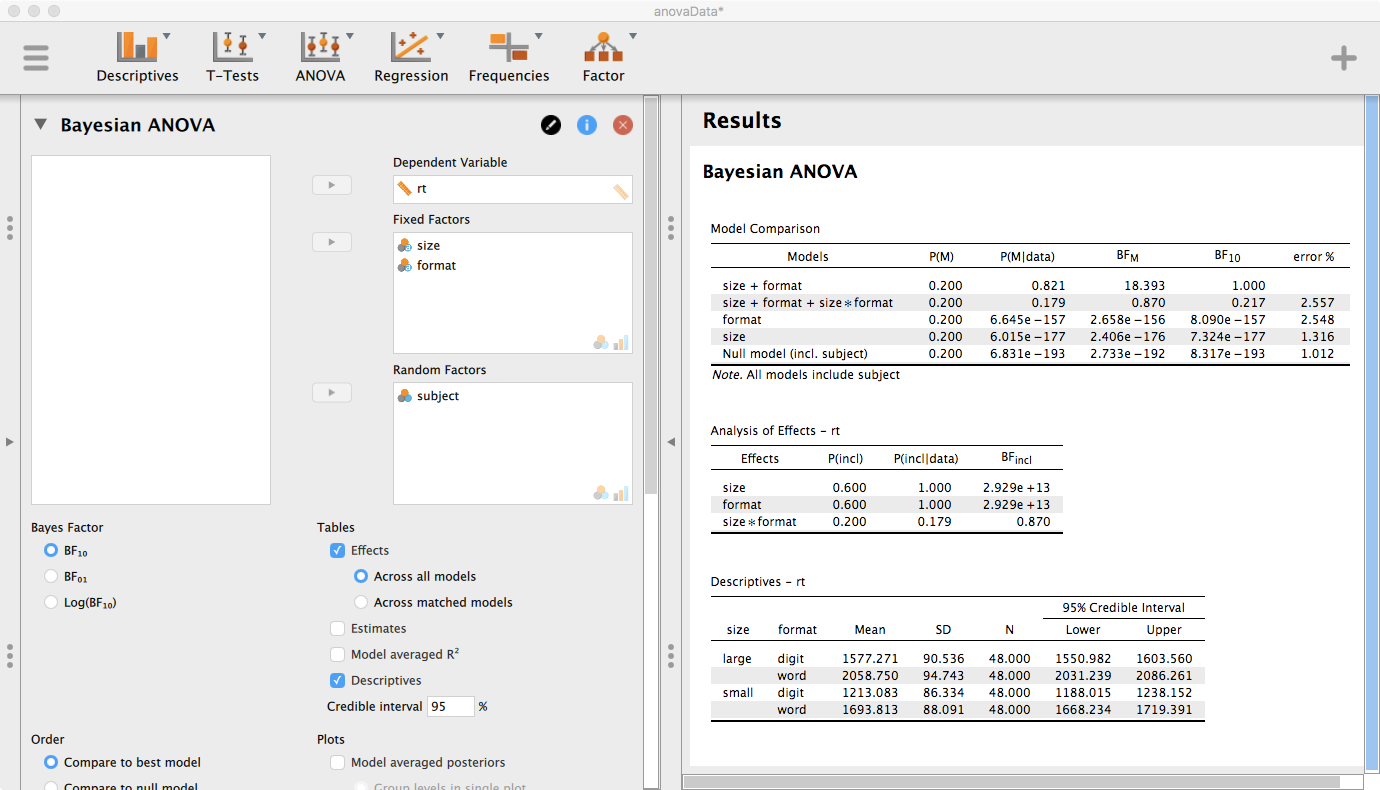
\includegraphics[width=0.9\textwidth,height=\textheight]{figures/anovaBayes.png}
\caption{\label{fig:anovaBayes}JASP screenshot showing a Bayesian analysis of variance.}
\end{figure}

The output shown in Figure \ref{fig:anovaBayes} will look similar to the linear regression example we did previously. Based on the fixed factors that are entered, JASP constructs a set of models to reflect the possible additive and interaction between these factors. Since we entered two fixed factors (size and format), JASP builds 5 competing models (all containing a random factor of \texttt{subject}:

\begin{align*}
  \mathcal{M}_{0}: & \text{ rt} = \text{ (null model)}\\
  \mathcal{M}_{1}: & \text{ rt} = \text{size} \text{ (main effect of problem size only)}\\
  \mathcal{M}_{2}: & \text{ rt} = \text{format} \text{ (main effect of format only)}\\
  \mathcal{M}_{3}: & \text{ rt} = \text{size}+\text{format} \text{ (additive model, no interaction)}\\
  \mathcal{M}_{4}: & \text{ rt} = \text{size}+\text{format}+\text{size*format} \text{ (interaction model)}\\
\end{align*}

These models are each displayed in the rows of the output in Figure \ref{fig:anovaBayes} in decreasing order of model fit (i.e., the best fitting model is listed at the top). We can see immediately that the best fitting model is \(\mathcal{M}_{3}\), the additive model without the interaction term. But, to understand why it is the best model and how it compares to the other 4 models, we need to discuss what each of the columns in the output table represent.

The first column, \(P(M)\), lists the prior probabilities of the 5 models. By default, JASP assigns these models to have equal probability, \emph{a priori}. Since there are 5 models, the prior probability of each model is \(1/5 = 0.2\). The second column, \(P(M\mid \text{data})\), gives the posterior model probabilities. Like the prior model probabilities, these must add to 1, but now there has been some shift from prior model probability to posterior model probability. Here, after observing data, we can see that the additive model \(\mathcal{M}_{3}\) and the interaction model \(\mathcal{M}_{4}\) account for most of our posterior belief (with posterior probabilities 0.821 and 0.179, respectively). The remaining three models essentially have posterior probability 0.

As in the regression example, the third column, \(\textnormal{BF}_{M}\), gives the factor by which the prior odds for a given model have been updated to produce the posterior odds for that model. For example, consider the additive model \(\mathcal{M}_{3}\). The prior odds for \(\mathcal{M}_{3}\), which is defined as the probability that \(\mathcal{M}_{3}\) is the true model divided by the probability that \(\mathcal{M}_{3}\) is \emph{not} the true model, can be computed as \(0.2/(1-0.2) = 0.2/0.8 = 0.25\). By similar calculation, the posterior odds are equal to \(0.821/(1-0.821) = 0.821/0.179 = 4.587\). Thus, the updating factor from prior odds to posterior odds is calculated as \(4.587/0.25 = 18.393\). One of the useful properties of this column is that it tells the user quickly whether the odds for a particular model has \emph{increased} or \emph{decreased}. As we can see in Figure \ref{fig:anovaBayes}, the only model for which model odds have increased is the additive model \(\mathcal{M}_{3}\).

Finally, the fourth column, \(\textnormal{BF}_{10}\), lists the Bayes factor for a given model compared to the best fitting model (note that this is the default setting in JASP, but if desired, it can be changed by the user to instead display the Bayes factor compared to the null model). This is a very useful column for the specific model comparison that is motivated by this example, namely the comparison of the additive model \(\mathcal{M}_{3}\) to the interaction model \(\mathcal{M}_{4}\). In the results table, we see that the Bayes factor for the interaction model \(\mathcal{M}_{4}\) compared to the additive model \(\mathcal{M}_{3}\) is 0.217. Taking reciprocals, this tells us that the Bayes factor for the additive model over the interaction model is \(1/0.217 = 4.61\). In other words, the observed data are approximately 5 times more likely under the additive model than under the interaction model, giving moderate support for an additive-only model of mental arithmetic.

The second table in the JASP results output simply recasts the results of the top table into a form that may translate better to researchers who are trained to think about ANOVA models as testing \enquote{effects}. If we think about the terms of the model as potential effects to test, we have three questions: do we include (1) a main effect of problem size; (2) a main effect of format; and (3) an interaction effect? This problem is cast in terms of \emph{inclusion probabilities}; i.e., what is the probability of including this term, or effect, in the best fitting model? Of course, the problem is Bayesian, so we have to think about how prior model probabilities are updated to posterior model probabilities after observing data. This information is summarized in three columns, described next.

The first column, \(P(\text{incl})\), lists the prior probability of including a particular term in the model. We can see that the prior probability of including \enquote{size} as a term in the model is 0.6, but let's see why this is the case. Recall above that we listed 5 possible models; note also that 3 of the 5 models contained the variable \enquote{size}. Thus, the prior probability of including size in our model is 3/5 = 0.6. The other prior inclusion probabilities can be computed similarly.

The second column, \(P(\text{incl}\mid\text{data})\), gives the posterior probabilities of including a particular term in the model, after observing data. As we can see, the posterior inclusion probabilities for the effects of both problem size and format are very large (JASP reports them as 1.000). On the other hand, the posterior probability of including the interaction term actually decreases to 0.179 after observing data. The third column, \(\textnormal{BF}_{\text{incl}}\), quantifies this change as the factor by which the prior odds of including the term (i.e., \(P(\text{incl})/P(\text{not incl}))\)) have changed to posterior inclusion odds after observing data. For both effects of problem size and format, this Bayes factor is extremely large, giving us overwhelming evidence for the \enquote{effects} of problem size and format. However, the prior odds for including an interaction term have decreased from \(0.2/(1-0.2) = 0.2/0.8 = 0.25\) to posterior odds of \(0.179/(1-0.179) = 0.179/0.821 = 0.218\), a factor of \(0.218/0.25 = 0.870\).

\hypertarget{conclusions}{%
\section{Conclusions}\label{conclusions}}

The examples provided in this tutorial represent a broad class of techniques that are common to many studies in numerical cognition and should be familiar to most researchers.

\begin{itemize}
\tightlist
\item
  reiterate benefits of Bayesian testing
\item
  give reference to other JASP and Bayes tutorials
\end{itemize}

\newpage

\hypertarget{references}{%
\section{References}\label{references}}

\setlength{\parindent}{-0.5in}
\setlength{\leftskip}{0.5in}

\hypertarget{refs}{}
\leavevmode\hypertarget{ref-bahadur2009optimality}{}%
Bahadur, R. R., \& Bickel, P. J. (2009). An optimality property of Bayes' test statistics. \emph{Lecture Notes-Monograph Series}, \emph{57}, 18--30.

\leavevmode\hypertarget{ref-bayarri2012criteria}{}%
Bayarri, M. J., Berger, J. O., Forte, A., \& Garcia-Donato, G. (2012). Criteria for Bayesian model choice with application to variable selection. \emph{The Annals of Statistics}, \emph{40}(3), 1550--1577.

\leavevmode\hypertarget{ref-campbellFugelsang2001}{}%
Campbell, J. I. D., \& Fugelsang, J. (2001). Strategy choice for arithmetic verification: Effects of numerical surface form. \emph{Cognition}, \emph{80}(3), B21--B30. doi:\href{https://doi.org/10.1016/s0010-0277(01)00115-9}{10.1016/s0010-0277(01)00115-9}

\leavevmode\hypertarget{ref-faulkenberry2019estimating}{}%
Faulkenberry, T. J. (2019). Estimating evidential value from analysis of variance summaries: A comment on ly et al.(2018). \emph{Advances in Methods and Practices in Psychological Science}, 2515245919872960.

\leavevmode\hypertarget{ref-gronauInpressinformed}{}%
Gronau, Q. F., Ly, A., \& Wagenmakers, E.-J. (n.d.). Informed Bayesian \(t\)-tests. \emph{The American Statistician}.

\leavevmode\hypertarget{ref-grunwald2019safe}{}%
Grünwald, P., Heide, R. de, \& Koolen, W. (2019). Safe testing. \emph{arXiv Preprint arXiv:1906.07801}.

\leavevmode\hypertarget{ref-hendriksen2018optional}{}%
Hendriksen, A., Heide, R. de, \& Grünwald, P. (2018). Optional stopping with Bayes factors: A categorization and extension of folklore results, with an application to invariant situations. \emph{arXiv Preprint arXiv:1807.09077}.

\leavevmode\hypertarget{ref-hollowayAnsari2009}{}%
Holloway, I. D., \& Ansari, D. (2009). Mapping numerical magnitudes onto symbols: The numerical distance effect and individual differences in children's mathematics achievement. \emph{Journal of Experimental Child Psychology}, \emph{103}(1), 17--29. doi:\href{https://doi.org/10.1016/j.jecp.2008.04.001}{10.1016/j.jecp.2008.04.001}

\leavevmode\hypertarget{ref-jaspSoftware}{}%
JASP Team. (2019). JASP (Version 0.11.1.0){[}Computer software{]}. Retrieved from \url{https://jasp-stats.org/}

\leavevmode\hypertarget{ref-jeffreys1948theory2}{}%
Jeffreys, H. (1948). \emph{Theory of probability} (2nd ed.). Oxford, UK: Oxford University Press.

\leavevmode\hypertarget{ref-jeffreys1961}{}%
Jeffreys, H. (1961). \emph{The Theory of Probability (3rd ed.)}. Oxford, UK: Oxford University Press.

\leavevmode\hypertarget{ref-johnson2010use}{}%
Johnson, V. E., \& Rossell, D. (2010). On the use of non-local prior densities in Bayesian hypothesis tests. \emph{Journal of the Royal Statistical Society: Series B (Statistical Methodology)}, \emph{72}(2), 143--170.

\leavevmode\hypertarget{ref-li2018mixtures}{}%
Li, Y., \& Clyde, M. A. (2018). Mixtures of g-priors in generalized linear models. \emph{Journal of the American Statistical Association}, \emph{113}(524), 1828--1845.

\leavevmode\hypertarget{ref-liang2008mixtures}{}%
Liang, F., Paulo, R., Molina, G., Clyde, M. A., \& Berger, J. O. (2008). Mixtures of g priors for Bayesian variable selection. \emph{Journal of the American Statistical Association}, \emph{103}(481).

\leavevmode\hypertarget{ref-lorch1990}{}%
Lorch, R. F., \& Myers, J. L. (1990). Regression analyses of repeated measures data in cognitive research., \emph{16}(1), 149--157. doi:\href{https://doi.org/10.1037/0278-7393.16.1.149}{10.1037/0278-7393.16.1.149}

\leavevmode\hypertarget{ref-ly2017replication}{}%
Ly, A., Etz, A., Marsman, M., \& Wagenmakers, E. (2019). Replication Bayes factors from evidence updating. \emph{Behavior Research Methods}, \emph{51}(6), 2498--2508. doi:\href{https://doi.org/https://doi.org/10.3758/s13428-018-1092-x}{https://doi.org/10.3758/s13428-018-1092-x}

\leavevmode\hypertarget{ref-ly2017tutorial}{}%
Ly, A., Marsman, M., Verhagen, A. J., Grasman, R. P. P. P., \& Wagenmakers, E.-J. (2017). A tutorial on Fisher information. \emph{Journal of Mathematical Psychology}, \emph{80}, 40--55. doi:\href{https://doi.org/https://doi.org/10.1016/j.jmp.2017.05.006}{https://doi.org/10.1016/j.jmp.2017.05.006}

\leavevmode\hypertarget{ref-ly2016harold}{}%
Ly, A., Verhagen, A. J., \& Wagenmakers, E. (2016). 201601Harold Jeffreys's default Bayes factor hypothesis tests: Explanation, extension, and application in psychology. \emph{Journal of Mathematical Psychology}, \emph{72}, 19--32. doi:\href{https://doi.org/http://dx.doi.org/10.1016/j.jmp.2015.06.004}{http://dx.doi.org/10.1016/j.jmp.2015.06.004}

\leavevmode\hypertarget{ref-moyer1967}{}%
Moyer, R. S., \& Landauer, T. K. (1967). Time required for judgements of numerical inequality. \emph{Nature}, \emph{215}(5109), 1519--1520. doi:\href{https://doi.org/10.1038/2151519a0}{10.1038/2151519a0}

\leavevmode\hypertarget{ref-rouder2012defaultRegression}{}%
Rouder, J. N., \& Morey, R. D. (2012). Default Bayes factors for model selection in regression. \emph{Multivariate Behavioral Research}, \emph{47}(6), 877--903.

\leavevmode\hypertarget{ref-rouder2012defaultAnova}{}%
Rouder, J. N., Morey, R. D., Speckman, P. L., \& Province, J. M. (2012). Default Bayes factors for ANOVA designs. \emph{Journal of Mathematical Psychology}, \emph{56}(5), 356--374.

\leavevmode\hypertarget{ref-rouder2009bayesian}{}%
Rouder, J. N., Speckman, P. L., Sun, D., Morey, R. D., \& Iverson, G. (2009). Bayesian t tests for accepting and rejecting the null hypothesis. \emph{Psychonomic Bulletin \& Review}, \emph{16}(2), 225--237.

\leavevmode\hypertarget{ref-vandeschoot2017systematic}{}%
van de Schoot, R., Winter, S. D., Ryan, O., Zondervan-Zwijnenburg, M., \& Depaoli, S. (2017). A systematic review of Bayesian articles in psychology: The last 25 years. \emph{Psychological Methods}, \emph{22}(2), 217--239.

\leavevmode\hypertarget{ref-vergutsDeMoor2005}{}%
Verguts, T., \& De Moor, W. (2005). Two-digit comparison: Decomposed, holistic, or hybrid? \emph{Experimental Psychology}, \emph{52}(3), 195--200. doi:\href{https://doi.org/10.1027/1618-3169.52.3.195}{10.1027/1618-3169.52.3.195}

\leavevmode\hypertarget{ref-wagenmakers2010}{}%
Wagenmakers, E.-J., Lodewyckx, T., Kuriyal, H., \& Grasman, R. (2010). Bayesian hypothesis testing for psychologists: A tutorial on the Savage--Dickey method. \emph{Cognitive Psychology}, \emph{60}(3), 158--189. doi:\href{https://doi.org/10.1016/j.cogpsych.2009.12.001}{10.1016/j.cogpsych.2009.12.001}

\leavevmode\hypertarget{ref-zellner1980posterior}{}%
Zellner, A., \& Siow, A. (1980). Posterior odds ratios for selected regression hypotheses. In J. M. Bernardo, M. H. DeGroot, D. V. Lindley, \& A. F. Smith (Eds.), \emph{Bayesian statistics: Proceedings of the first international meeting held in Valencia} (Vol. 1, pp. 585--603). Springer.


\end{document}
